%%%%%%%%%%%%%%%%%%% vorlage.tex %%%%%%%%%%%%%%%%%%%%%%%%%%%%%
%
% LaTeX-Vorlage zur Erstellung von Projekt-Dokumentationen
% im Fachbereich Informatik der Hochschule Trier
%
% Basis: Vorlage svmono des Springer Verlags
%
%%%%%%%%%%%%%%%%%%%%%%%%%%%%%%%%%%%%%%%%%%%%%%%%%%%%%%%%%%%%%

\documentclass[envcountsame,envcountchap, deutsch]{i-studis}

\usepackage{makeidx}         	% Index
\usepackage{multicol}        	% Zweispaltiger Index
%\usepackage[bottom]{footmisc}	% Erzeugung von Fu�noten

%%-----------------------------------------------------
%\newif\ifpdf
%\ifx\pdfoutput\undefined
%\pdffalse
%\else
%\pdfoutput=1
%\pdftrue
%\fi
%%--------------------------------------------------------
%\ifpdf
\usepackage[pdftex]{graphicx}
\usepackage{epstopdf}
\usepackage[pdftex,plainpages=false]{hyperref}
%\else
%\usepackage{graphicx}
%\usepackage[plainpages=false]{hyperref}
%\fi

%%-----------------------------------------------------
\usepackage{color}				% Farbverwaltung
%\usepackage{ngerman} 			% Neue deutsche Rechtsschreibung
\usepackage[english, ngerman]{babel}
\usepackage{enumitem}
%\usepackage[latin1]{inputenc} 	% Erm�glicht Umlaute-Darstellung
\usepackage[utf8]{inputenc}  	% Erm�glicht Umlaute-Darstellung unter Linux (je nach verwendetem Format)

%-----------------------------------------------------
\usepackage{listings} 			% Code-Darstellung
\lstset
{
	basicstyle=\ttfamily,	% print whole listing small
	keywordstyle=\color{blue}\bfseries,
	frame=single,
	columns=fullflexible,
								% underlined bold black keywords
	identifierstyle=, 			% nothing happens
	commentstyle=\color{red}, 	% white comments
	stringstyle=\ttfamily, 		% typewriter type for strings
	showstringspaces=false, 	% no special string spaces
	framexleftmargin=7mm, 
	tabsize=3,
	showtabs=false,
	frame=single, 
	rulesepcolor=\color{blue},
	numbers=left,
	linewidth=146mm,
	xleftmargin=8mm,
	breaklines=true,
	postbreak=\mbox{\textcolor{red}{$\hookrightarrow$}\space},
}

\usepackage{textcomp} 			% Celsius-Darstellung
\usepackage{amssymb,amsfonts,amstext,amsmath}	% Mathematische Symbole
\usepackage[german, ruled, vlined]{algorithm2e}
\usepackage[a4paper]{geometry} % Andere Formatierung
\usepackage{bibgerm}
\usepackage{array}
\usepackage{caption}
\hyphenation{Ele-men-tar-ob-jek-te  ab-ge-tas-tet Aus-wer-tung House-holder-Matrix Le-ast-Squa-res-Al-go-ri-th-men} 		% Weitere Silbentrennung bei Bedarf angeben
\setlength{\textheight}{1.1\textheight}
\pagestyle{myheadings} 			% Erzeugt selbstdefinierte Kopfzeile
\makeindex 						% Index-Erstellung


%--------------------------------------------------------------------------
\begin{document}
%------------------------- Titelblatt -------------------------------------
\title{Natural Language Processing und Text übersetzung}
\subtitle{Natural Language Processing and Text Translation}
%---- Die Art der Dokumentation kann hier ausgew�hlt werden---------------
%\project{Bachelor-Projektarbeit}
%\project{Bachelor-Abschlussarbeit}
%\project{Master-Projektstudium}
\project{Master-Abschlussarbeit}
%\project{Seminar zur Vorlesung ...}
%\project{Hausarbeit zur Vorlesung ...}
%--------------------------------------------------------------------------
\supervisor{Prof. Dr. Hans Beise} 		% Betreuer der Arbeit
\author{Bachvarov, Vladislav} 							% Autor der Arbeit
\address{Trier,} 							% Im Zusammenhang mit dem Datum wird hinter dem Ort ein Komma angegeben
\submitdate{Abgabedatum} 				% Abgabedatum
%\begingroup
%  \renewcommand{\thepage}{title}
%  \mytitlepage
%  \newpage
%\endgroup
\begingroup
  \renewcommand{\thepage}{Titel}
  \mytitlepage
  \newpage
\endgroup
%--------------------------------------------------------------------------
\frontmatter 
%--------------------------------------------------------------------------
\preface

Ein Vorwort ist nicht unbedingt n�tig. Falls Sie ein Vorwort schreiben, so ist dies der Platz, um z.B. die Firma vorzustellen, in der diese Arbeit entstanden ist, oder einigen Leuten zu danken, die in irgendeiner Form positiv zur Entstehung dieser Arbeit beigetragen haben. Auf keinen Fall sollten Sie im Vorwort die Aufgabenstellung n�her erl�utern oder vertieft auf technische Sachverhalte eingehen.				% Vorwort (optional)


\kurzfassung
\inputencoding{latin1}
\paragraph*{}

Diese Arbeit befasst sich mit dem Thema Natural-Language-Processing (NLP), pr�ziser gesagt Transformer. In den ersten Kapiteln der Arbeit wird eine Einf�hrung in das Thema Vektorrepr�sentation von W�rtern gegeben. Nachfolgend werden die Modelle Transformer und BERT erkl�rt und schlie�lich wird die Struktur als Programmcode dargestellt. Das letzte und wichtigste Kapitel verschafft einen �berblick �ber Neural-Machine-Translation und die Anwendung solcher Modelle f�r die �bersetzung. Anschlie�end werden diese Modelle untersucht und eine Schlussfolgerung anhand der Ergebnisse wird gezogen.

%% deutsch
%\paragraph*{}
%In der Kurzfassung soll in kurzer und pr�gnanter Weise der wesentliche Inhalt der Arbeit beschrieben werden. Dazu z�hlen vor allem eine kurze Aufgabenbeschreibung, der L�sungsansatz sowie die wesentlichen Ergebnisse der Arbeit. Ein h�ufiger Fehler f�r die Kurzfassung ist, dass lediglich die Aufgabenbeschreibung (d.h. das Problem) in Kurzform vorgelegt wird. Die Kurzfassung soll aber die gesamte Arbeit widerspiegeln. Deshalb sind vor allem die erzielten Ergebnisse darzustellen. Die Kurzfassung soll etwa eine halbe bis ganze DIN-A4-Seite umfassen.
%
%Hinweis: Schreiben Sie die Kurzfassung am Ende der Arbeit, denn eventuell ist Ihnen beim Schreiben erst vollends klar geworden, was das Wesentliche der Arbeit ist bzw. welche Schwerpunkte Sie bei der Arbeit gesetzt haben. Andernfalls laufen Sie Gefahr, dass die Kurzfassung nicht zum Rest der Arbeit passt.

%% englisch
%\paragraph*{}
%The same in english.
 			% Kurzfassung Deutsch/English
\tableofcontents 						% Inhaltsverzeichnis
%\listoffigures 							% Abbildungsverzeichnis (optional)
%\listoftables 							% Tabellenverzeichnis (optional)
%--------------------------------------------------------------------------
\mainmatter                        		% Hauptteil (ab hier arab. Seitenzahlen)
%--------------------------------------------------------------------------
% Die Kapitel werden in separaten .tex-Dateien abgelegt und hier eingebunden.
\chapter{Einleitung und Problemstellung}

Begonnen werden soll mit einer Einleitung zum Thema, also Hintergrund und Ziel erl�utert werden.

Weiterhin wird das vorliegende Problem diskutiert: Was ist zu l�sen, warum ist es wichtig, dass man dieses Problem l�st und welche L�sungsans�tze gibt es bereits. Der Bezug auf vorhandene oder eben bisher fehlende L�sungen begr�ndet auch die Intention und Bedeutung dieser Arbeit. Dies k�nnen allgemeine Gesichtspunkte sein: Man liefert einen Beitrag f�r ein generelles Problem oder man hat eine spezielle Systemumgebung oder ein spezielles Produkt (z.B. in einem Unternehmen), woraus sich dieses noch zu l�sende Problem ergibt.

Im weiteren Verlauf wird die Problemstellung konkret dargestellt: Was ist spezifisch zu l�sen? Welche Randbedingungen sind gegeben und was ist die Zielsetzung? Letztere soll das
beschreiben, was man mit dieser Arbeit (mindestens) erreichen m�chte.
\chapter{Word2Vec}

In dieser Kapitel wird das Verfahren "Word2Vec" durch die Nutzung von Neuronalem Netz vorgestellt. Word2Vec ist eine Darstellung von Wörtern mit Vecoren, was auch aus die Abkürzung klar wird - Word ist klar; 2 - to; und Vec - Vector und das ganze "word to vector". Dieses Model ist am meisten  in der Natural Laguage Processing (NLP) verbreitet und wird in vielen Bereichen der Informatik genutzt, unter anderem in Spamfilterung und Dokumentenanalyse. Jedoch diese Technik besagt nur wie die Wörter eines Textes dargestellen werden können. Das Verfahren, bei dem die möglichst passenden Vektoren in einem ausgewählten Text, auch Corpus genant, gelernt werden, heißt Word Embeddings. Bei dieser Technik wird ein Neuronales Netzt eigesetzt. Die Vorgehensweise und die Idee wird folglich erklärt.

\section{Word Embedding}

Wie es schon in der Einleitung erwähnt wurde, Word Embedding ist der Prozess, bei dem die Wörter eines Textes in mathematischen Vektoren gewandelt werden. Zuerst muss der Corpus vorbeiretet werden. Ich stelle hier nur die Theorie und in einer späteren Kapitel (!? WICHTIG WELCHE GENAU!?) gehe ich tiefer in dem Programmcode.

\!!! DAS HIER GEHÖRT IN EINE ANDERE KAPITEL !!!
!!! DIE KAPITEL FÜR TEXTVORBEREITUNG ODER SOWAS!!!

Als der Text vorbeitet ist, sodass es von Sonderzeichen und alle unnötigen Zeichen bereinigt wird. Wenn der Text vorbeireitet ist, werden die Wörter aus dem Corpus bestimmt und jeder erhält einen Index. Üblicherweise werden die Wörter nach ihrer Häufigkeit angeordnet. Das häufigste Wort erhält somit den Index 1. Als nächstes werden die Wörter im Korpus durch ihren Index ersetzt, um alle Trainingspaare fürs Lernen generiert zu werden. Dies erfolgt in dem es durch das Corpus iteriert und in einem bestimmten Fenster, oder in der Literatur auch als Window gezeichnet, alle Contextwörter und den Targetwort ausgelesen werden. Das Targetwort ist das Wort in der Mitte, während die Wörter um das Targetwort entsprechend die Kontextwörter. 

!!! BIS HIER MUSS WEG !!!!

In der Literatur werden zwei Arten von Wort2Vec Modelle - SKIP-gram und CBOW (Continous Bag of Words). Beide Modelle verwenden ein Neuronales Netz mit einem oder zwei versteckten Schichten (siehe !!KAPITEL MIT DEM PROGRAMMCODE!!). Die beiden Methoden unterscheiden sich nach ihren Ein- und Ausgaben.   

\subsubsection{SKIP-gram Model}
Bei dem SKIP-gram-Model fließen die Targetwörter als Eingabe und das Model versucht ein Kontextwort zu raten. Hier ist die Struktur eines Skip-gram Models:

\begin{figure}
	\centering
	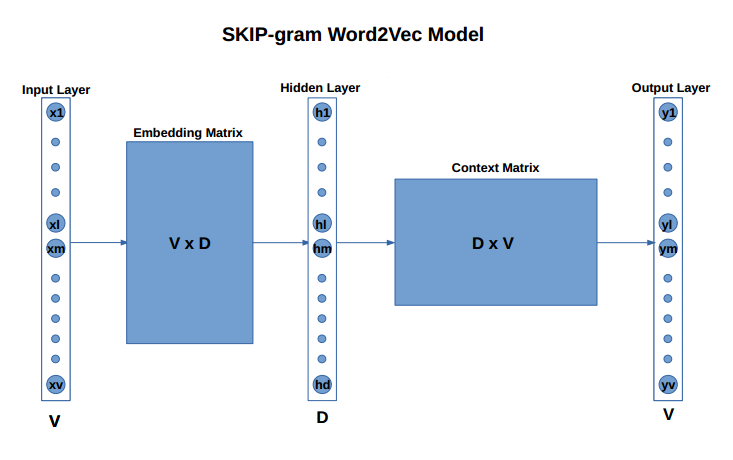
\includegraphics[scale=0.5]{images/SKIP_Model.png}
	\caption{Skip-gram Word2Vec Model}
	\label{skip}
\end{figure}

Aus der Abbildung \ref{skip} ist es zu entnehmen, dass ein Skip-gram Model aus einer hidden Schicht und zwei Eigabeschichten. Die Eingabe sowie die Ausgabe ist ein Vektor, der aus $\emph{V}$ Componente besteht. Das entspricht die größe des Wörterbuchs (engl. Vocabulary). Das versteckte Schicht besteht aus $\emph{D}$ Variablen und stellt einen Vektor dar. Die Dimensionalität dieses Vektors nimmt üblich einen Wert zwischen 25 und 300. Diese Variablen können auch als Eigenschaften für die Wörter betrachtet werden. Je mehr Kriterien es untersucht werden, desto besser die Beziehung zwischen Wörtern wiederspiegelt werden kann. Die Ausgabe ist wieder einen $\emph{V-dimensionalen}$ Vektor. Jedoch die Ausgabe ist kein One-Hot Vektor mehr, der das Kontextwort wiedergibt, sondern einen Wahrscheinlichkeitsvektor, dass der Wort mit der entsprechenden Index der richtige Contextwort ist.

Die zwei Matrizen sind identisch, jedoch die Kontextmatrize ist die transponierte Embeddingsmatrize. Diese Matrix beinhaltet unsere Wortvektoren.

Der Abbildung \ref{skip} nach besteht das neuronale Netz aus drei Schichten. Im Hiddenlayer steht ein Vektor, der abhängig von unsere Eingabe den Wortvektor repräsentiert. Die Ausgabe ist ein softmax

\subsubsection{CBOW Model}
Die Kontextwörter sind die Eingabe in dem CBOW-Model und das Model ratet der Targetwort. Die zwei Modelle besitzen die gleiche Anzahl an Schichten. Das CBOW-Model ist ein umgedrehtes SKIP-gram-Model, jedoch die Eingabe besteht aus $\emph{w}$-Viele Vektoren statt nur eins. Als nächstes stellt die \ref{cbow} Abbildung die beschriebene Struktur.

\begin{figure}
	\centering
	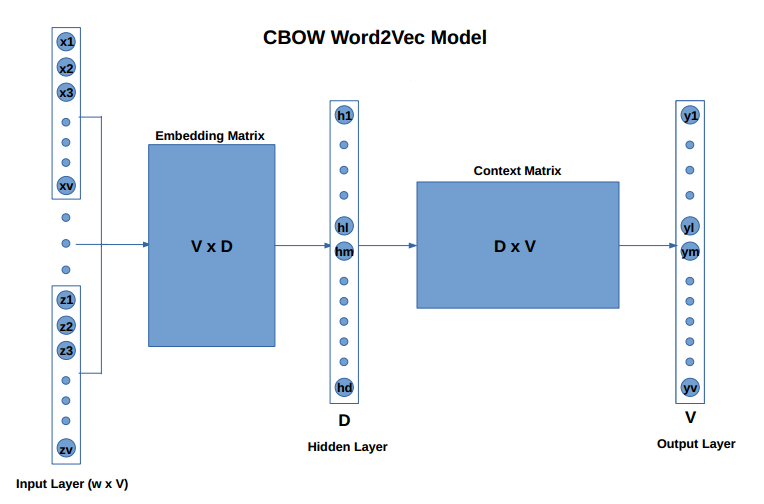
\includegraphics[scale=0.5]{images/CBOW_Model.png}
	\caption{CBOW Word2Vec Model}
	\label{cbow}
\end{figure}

Die Struktur des CBOW-Models besteht wieder aus eine Matrix für das Embedding der Target- und Kontextwörter. Die größe der Matrizen hängt von der ausgewählten Hyperparameter und die Größe des Datensatzes. Die Anzahl der verwendeten Inputvektoren entspricht die größe des gesetzten Window (Kontextfenster).

\subsection{Implementierung}
\chapter{GloVe}

Die Idee von \textbf{Glo}bal \textbf{Ve}ctors ist es, den Sinn hinter einem Wort in numerischer Vektorform darzustellen. GloVe ist eine weitere Möglichkeit neben word2vec(\cref{word2vec}) wie man Wörter oder sogar ganze Texte als Vektoren repräsentiert.

\section{GloVe-Methode}
Einige Variablen werden zuerst eingeleitet. Die Matrix der Word-Word-co-occu-rrence wird mit \textbf{$X$} notiert und eine beliebige Komponente in der Matrix mit \textbf{$X_{ij}$}. Der Wert \textbf{$X_{ij}$} stellt dar, wie oft das Wort \textit{j} in dem Kontext vom Wort \textit{i} vorkommt. Weiterhin beschreibt die Einheit \textbf{$X_i$} die Anzahl des Vorkommens eines beliebigen Wortes in dem Kontext vom Wort \textit{i} und ist in der folgenden \cref{x_i} definiert:

\begin{equation}
	X_i = \sum_{k} X_{ik}. \cite{GloVe:14}
	\label{x_i}
\end{equation}

Schließlich definieren wir die Einheit \textbf{$P_{ij}$}, die beschreibt, wie hoch die Wahrscheinlichkeit ist, dass ein Wort \textit{j} in dem Kontext vom Wort \textit{i} vorkommt. Die Formel ist in der \cref{p_ij} aufgeführt:

\begin{equation}
	P_{ij} = P(j|i) = \frac{X_{ij}}{X_i}. \cite{GloVe:14}
	\label{p_ij}
\end{equation}

Ein kleines Beispiel wird angegeben, damit verstanden werden kann, wie bestimmte Aspekte aus dem gemeinsamen Auftreten von Wörtern gewonnen werden können. Es werden zwei Wörter \textit{i} und \textit{j} betrachtet, die in einem Corpus vorkommen. Das Beispiel stammt aus dem Artikel \cite{GloVe:14} und ist aus dem Themenbereich des thermodynamischen Zustands. Nehmen wir die Wörter \textit{$i = ice$} und \textit{$j = steam$}. Die Beziehung der beiden Wörter kann so untersucht werden, indem die Relation mit anderen Probewörtern \textit{k} berechnet wird. Für Wörter, die in direktem Bezug zu \textit{$i = ice$} stehen, erwarten wir, dass das Verhältnis $\frac{P_{ik}}{P_{jk}}$ groß ist, zum Beispiel wenn das Wort \textit{$k = solid$} gewählt wird. Analoge Beziehung kann bei Wörtern betrachtet werden, die näher an Bedeutung zu \textit{$j = steam$} stehen. In solchen Fällen werden wir einen kleineren Wert des Bruchs $\frac{P_{ik}}{P_{jk}}$ erhalten - zum Beispiel wählen wir das Wort \textit{$k = gas$}. Selbstverständlich ist der Wert des Bruchs gleich eins, wenn das Wort \textit{k} zu beiden Wörtern \textit{i, j} in Korrelation steht, oder wenn sich keine Korrelation ergibt. Als Beispiel können wir das Wort \textit{$k = sun$} wählen. Die \cref{ice_steam_tab} stellt das Verhältnis zwischen den Wörtern dar:

	\begin{table}[]\label{tab_1}
		\centering
		\begin{tabular}{l|l|l|l|l}
			Probability and Ration & k = solid                                           & k = gas                                             & k = water                                           & k = fashion                                         \\ \hline
			P(k|ice)               & 1.9\times 10^{-4} & 6.6\times 10^{-5} & 3.0\times 10^{-3} & 1.7\times 10^{-5} \\
			P(k|steam)             & 2.2\times 10^{-5} & 7.8\times 10^{-4} & 2.2\times 10^{-3} & 1.8\times 10^{-5} \\
			P(k|ice)/P(k|steam)    & 8.9                                                 & 8.5\times 10^{-2} & 1.36                                                & 0.96                                               
		\end{tabular}
		\captionof{table}{Tabelle von dem Vorkommen der beiden Wörter \textit{ice} und \textit{steam} \cite{GloVe:14}}\label{ice_steam_tab}
	\end{table}
 
Die Erwartungen werden durch die \cref{ice_steam_tab} gerechtfertigt. Die Rate erlaubt uns, die Verhältnisse zwischen den einzelnen Wörtern besser zu verstehen. Mit Hilfe des Bruches wird unterschieden, wie die Wörter zueinander stehen, im Gegensatz zu der einfachen Wahrscheinlichkeit.

Zu betrachten ist, dass die Wahrscheinlichkeit der Koinzidenz von drei Eingangsgrößen \textit{i}, \textit{j}, \textit{k}, abhängt. Die Allgemeinform der Funktion ist in der \cref{alg_f} angegeben:

\begin{equation}
	F(w_i, w_j, \~w_k) = \frac{P_{ik}}{P_{jk}} \cite{GloVe:14}.
	\label{alg_f}
\end{equation}

Die Wortvektoren für untersuchte Wörter \textit{i,j} sind durch \textit{w} $\in$ $\mathbb{R^d}$ gegeben und das betrachtete Wort {k} ist mit Vektor \textit{\~w} $\in$ $\mathbb{R^d}$ repräsentiert. In der Gleichung entsteht die rechte Seite aus dem Corpus (Vocabulary). F hängt in diesem Fall von den drei Vektoren $w_i, w_j, \~w_k$ ab. F wird im nächsten Schritt wegen der hohen Variation der Formel angepasst. Zuerst ist es gewünscht, die Information aus der Rate in Word-Vector-Raum darzustellen. Da Vektorräume ursprünglich linear sind, kann dies in einer Vektordifferenz erfolgen. Somit fällt der Fokus nur auf die Funktionen, die von der Differenz der zwei Vektoren abhängen. Die Änderung wird aus der \cref{f_dif} ersichtlich.

\begin{equation}
F((w_i - w_j), \~w_k) = \frac{P_{ik}}{P_{jk}} \cite{GloVe:14}.
\label{f_dif}
\end{equation}

Für die Gleichung ist es zu erwähnen, dass die Parameter von F Vektoren sind, während die rechte Seite ein Skalar ist. Während \textit{F} als eine komplexere Funktion, die von einem neuronalen Netz parametrisiert werden kann, genommen werden kann, würde das die Linearstruktur der Formel verschleiern. Es wird das Skalarprodukt genommen, damit die Verschleierung vermieden wird. Die \cref{f_dot} stellt die Änderung dar.
\begin{equation}
F((w_i - w_j)^T\~w_k) = \frac{P_{ik}}{P_{jk}} \cite{GloVe:14}.
\label{f_dot}
\end{equation}

Laut \cite{GloVe:14} erfolgt in der word-word Koinzidenzmatrizen der Unterschied zwischen Wort und Kontextwort willkürlich. Die Formel für F muss erlauben, dass zwei Rollen beliebig ausgetauscht werden können. Das heißt also nicht nur $w \leftrightarrow \~w$ auszutauschen, sondern auch $X \leftrightarrow X^T$. Um diese Symmetrie zu verschaffen, sind zwei einfache Schritte erforderlich. Zuerst muss sichergestellt werden, dass die Formel homomorphisch zwischen den Gruppen ($\mathbb{R}$, +) und ($\mathbb{R}_{>0}$, $\times$) ist:

\begin{equation}
F((w_i - w_j)^T\~w_k) = \frac{F(w_i^T\~w_k)}{F(w_j^T\~w_k)} \cite{GloVe:14},
\label{f_hom}
\end{equation}	

was nach \cref{f_dot} wie folgt aussieht:

\begin{equation}
F(w_i^T\~w_k) = P_{ik} =\frac{X_{ik}}{X_i} \cite{GloVe:14}.
\label{f_hom_res}
\end{equation}

Die Lösung von \cref{f_hom} ist $F = exp$, oder auch:

\begin{equation}
w_i^T\~w_k = \log (P_{ik}) = \log(X_{ik}) - \log(X_i) \cite{GloVe:14}.
\label{f_hom_sol}
\end{equation}

Zunächst wird die Gleichung umgestellt, jedoch werden einige Konstanten eingeführt. Es könnte der Wert von $\log(X_i)$ in einer Konstante $b_i$ umgewandelt werden. Schließlich wird die Konstante $b_k$ addiert, damit die Symmetrie erhalten wird. Die vereinfachte Formel ist in der \cref{f_simp} gegeben:

\begin{equation}
w_i^T\~w_k + b_i + \~b_k = \log(X_{ik}) \cite{GloVe:14}.
\label{f_simp}
\end{equation}

Nach der Einführung in Wortvektoren steigen wir in den nächsten Kapiteln ins Hauptthema Transformer ein. Die Folgekapitel erläutern die Struktur und Implementierung von dem Transformer und \textbf{B}idirectional \textbf{E}ncoder \textbf{R}epresentation from \textbf{T}ransformer (oder kurz BERT). Schließlich wird ein Modell vorgestellt, das versucht die Hauptaufgabe dieser Ausarbeitung zu lösen.


\chapter{Der Transformer} \label{Transformer}

In der zweiten Hälfte des Jahres 2017 ein Team von Wissenschaftlern veröffentlichte ihr Papier \textquotedblright Attention Is All You Need\textquotedblright, in dessen sie ein neues Model vorstellten. Das Projekt zur Entwicklung wurde unter der Google Research and Google Brain aufgeführt. Dieses Model nahm die Name der "Transformer".

\section{Struktur des Transformers}
Der Transformer besteht aus zwei Haupteinheiten, deren Namen Encoder und Decoder sind. Die beiden Einheiten bestehen aus gleicher Anzahl Encoder-, bzw. Decoder-, Layers. Der im Pappier vorgestellte Encoder verfügte über 6 Encoderschichten und 6 Decoderschichten. Die folgende Abbildung beschreibt den Transformer:


\begin{figure}
	\centering
	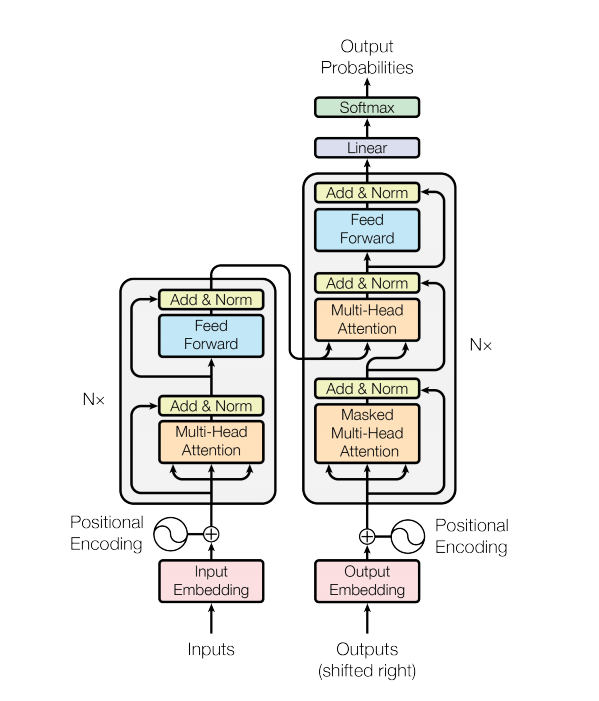
\includegraphics[scale=0.36]{images/transformer.png}
	\caption{Das Transformer-Modell}
	\label{transformer}
\end{figure}

In den linken Schichten fließt der Input, meistens mehrere Sätze, durch eine Attention- und eine FeedForward-Network(FFN) Unterschicht. Rechts werden die Targeteingaben, die zugehörigen Sätze für den Input, von zwei Attention- und wieder von einer FFN-Unterschichten. Der Input- und der Targetsatz werden eingebettet, before sie in den Encoder, bzw. Decoder, eingegeben worden. Zuerst werden die einzelnen Wörter der Sätze durch ihre entsprechende Kodierung in Zahlen ersetzt. Demnächst wird eine Positionale Kodierung in der Eingabe eingebettet.

Die nächsten Unterkapitel betrachten die einzelnen Aufbauelementen des Transformers ins Details. Wichtig ist es Hier zu erwähnen, dass die Positionale Einbettung von keiner Einheit im Transformer durchgeführt ist, sondern eine zusätzliche Vorbearbeitung des Textes (Text Preprocessing). Jedoch erkläre ich die Mathematik, die dahinter steckt.

\subsection{Positionale Einbettung}
Die Positionale Einbettung passiert nach der Umwandlung von Text in Zahlen. Wie die Name erratet, wird Information über die Lage des Wortes im Satz in den Wortvektor eingebettet. Diese zusätliche Aktion ist notwig, da im vergleich zu anderen Modelle oder Verfahren, beihaltet der Transformer keine Convolutional- oder Recurenz-Netzwerke.

Die Formel nach dem der Vektor berechnet wird, ist gegeben:

\begin{equation}
	PE_{(pos,2i)} = \sin\Bigg(\frac{pos}{10000^\frac{2i}{d_{model}}}\Bigg)
\end{equation}
\begin{equation}
	PE_{(pos,2i+1)} = \cos\Bigg(\frac{pos}{10000^\frac{2i}{d_{model}}}\Bigg)
\end{equation}

Der PE-Vektor besteht aus $d_model$-Dimensionen. Für jede Dimension wird der Wert des Eintrages entweder mit der Sinus oder der Cosinus-Funktion berechnet. Die geraden Dimensionen entsprechend mit der Sinusfunktion und die Ungeraden mit der Cosinusfunktion.

Als nächstes wird betrachtet, wie der PE-Vektor zum Einbettungs-Vektor addiert wird. In der Literatur werden die Vektoren ganz einfache addiert. Diese Vorgehensweise könnte jedoch Probleme verursachen und wichtige Informationen könnten verloren gehen. Es existieren mehrere Möglichkeiten, wie man das Verlust von Informationen zu vermeiden. Im Buch \cite{denis_Transformer:02} wird folgende Formel benutzt:

\begin{equation}
	pc(i) = y_i*math.sqrt(d_{model}) + pe(i)
\end{equation}

,wo der Eingabevektor durch eine Konstante skaliert wird. Die Variable $y_i$ ist der eingebettete Vektor und $pe$ ist der Positionalsvektor und $d_{model}$ entspricht die Anzahl der Dimensionen des Vektoren benutzt im Model. Der Eingabevektor wird mit dem Wurzel vom Dimensionen skaliert und erst dann wird der Positionalvektor addiert.

\subsection{Encoder und Decoder}

Encoder und Decoder sind die essenziellen Bestandteile vom Transformer. Der Encoder erhält die schon veränderten Daten und führt sie durch ein Attention- und ein Feed Forward Network-Layer. Zwischen jeder Unterschicht besteht eine residierte Verbindung (siehe Abbildung \ref{transformer}), sodass die Ausgaben vom letzten Unterlayer mit den Ausgaben vom Aktuellen addiert und weiterhin normiert werden. Der Decoder besitzt eine Unterschicht mehr als der Encoder. In der Transformer beinhaltet der Decoder drei Schichten (siehe Abbildung \ref{transformer}). Die letzten zwei sind die selben wie im Encoder. Die erste Unterschicht im Decoder ist eine Masked-Multi-Head-Attention-Schicht. Die Verbindung zwischen Encoder und Decoder erfolgt in der zweiten Unterschicht - zwar in der MHA-Schicht. Da werden die Ausgaben vom Encoder und vom MMHA-Schicht zusammengeführt. Nach der Bearbeitung liefert das Model einen potenziellen Satz, der abhängig vom Aufgaben Stellung, die gesuchte Antwort sein sollte. In diesem Fall ist es die Übersetzung aus dem Englishen ins Spanische. In den folgenden Unterkapiteln werden die Unterschichten ins Details untersucht.

\subsubsection{Multi-Head-Attention Layer}
Der Multi-Head-Attention Layer kommt in den beiden Einheiten vor. Dieser Schicht folgt eine Normierungsschicht, die die Ausgaben aus dem MHA-Schicht und die Residial-Daten aus vorheriger Schicht addiert und normiert.

Die Eingabe in dem Multi-Head-Attention-Layer vom Encoder ist der Vektor, der die positionale und eingebettete Angaben vom Text erhählt. Im Decoder erhält der MHA-Layer die Eingaben von einer Masked-Multi-Head-Attention-Schicht, und somit ist die Information bis zum aktuell betrachteten Punkt. Der unteschied besteht darin, dass die Information für den Encoder komplett verfügbar ist, und im Decoder wird diese maskiert, und so lernt das Model zu raten. Darin besteht der Unterschied zwischen den MHA im Encoder und Decoder. 

Ziel dem MHA-Layer im Encoder` ist es die Bezihung zwischen einzelnen Worten zu bestimmen. Das wird erzielt, indem jedes Wort aus dem Satz mit allen anderen abgebildet wird. Jedoch  Jedes Wortvektor besteht aus $d_{model}$ Dimensionen. In dem Buch \cite{denis_Transformer:02} entspricht die Anzahl an Dimensionen gleich 512. Die große Anzahl der Dimensionen würde große Laufzeit anfordern, wenn mehrere Ansichten untersucht werden wollen. Dies ist natürlich möglich mit den stärken Komputern von heute. Der Nachteil ist natürlich, dass das Model immer nur eine Ansicht über die Beziehungen der Wörter betrachtet und es natürlich noch mehr Leistung erfordern würde, um weitere Ansichten zu bestimmen. Eine bessere Alternative ist die Dimensionen jedes Wortes in 8 Teilen, jedem Teil (auch Head genannt im \cite{denis_Transformer:02}) entspricht 64 Dimensionen, aufzuteilen. Dann wird jeder 64-stückige Teil den 8 unterschiedlichen Heads (deswegen ist die Schicht Multi-Head-Attention-Layer genannt; siehe Abbildung \ref{multi_head}) zum untersuchen gegeben. 

\begin{figure}
	\centering
	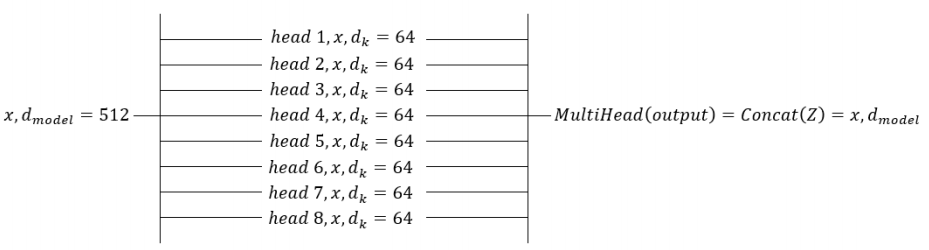
\includegraphics[scale=0.4]{images/multi_head.png}
	\caption{Heads \cite{denis_Transformer:02}}
	\label{multi_head}
\end{figure}

Diese ``Köpfe'' laufen parallel. Der Vorteil dabei ist es, dass die Laufzeit verringert wird und es 8 unterschiedliche Repräsentationen betrachtet werden. In der Abbildung \ref{multi_head} erkennt man wie die MHA-Schicht aussieht. Nachdem die Daten von jedem Kopf vorhanden sind, werden die Ergebnisvektoren wieder konkateniert (siehe Abbildung \ref{multi_head}). Die Ausgabe sieht, dann wie folgt aus:

\begin{equation}
	Z = (z_0, z_1, z_2, z_3, z_4, z_5, z_6, z_7)
\end{equation}

Die Matrix Z ist die aus den Ausgaben $z_i$ aufgebaute Ergebnismatrix. Am Ende muss die Matrix $Z$ zusätzlich konkateniert werden, um die ursprünglichen Dimensionen $x*d_{model}$ zu erhalten.

In jedem Kopf wird jedes Wort mit drei Vektoren repräsentiert:
\begin{itemize}
	\item Einem Query-Vektor ($Q$), dessen Dimensionalität $d_q$ gleich \textbf{64} ist. Der Vektor wird verwendet, oder trainiert, wenn der zugehörige Wortvektor für $x_n$ die Key-Value-Paare gesucht sind, inklusive sich selbst.
	
	\item Einem Schlüsselvektor (auch als Key-Vektor bezeichnet $K$), der trainiert wird, um einen Attention-Wert zu ergeben.
	
	\item Einem Wertvektor (auch als Value-Vektor bezeichnet $V$), der trainiert wird, um einen weitere Anttention-Wert zu ergeben.
\end{itemize}

Im Buch \cite{denis_Transformer:02} wird das Attention als "Scaled Dot-Product Attention" bezeichnet. Das ist eine Linearkombination der oben deklarierten Vektoren. Die folgende Formel ergibt seine Berechnung: 

\begin{equation}
	Attention(Q, K, V) = softmax\Bigg(\frac{Q*K^T}{\sqrt{d_k}}\Bigg)* V
\end{equation}

Diese Vektorrepräsentationen werden aus den Gewichtsmatrizen eingelesen. Die Gewichtsmatrizen, sind am Anfang nicht bekannt und werden im Folge der Training bestimmt. Zu Beginn werden sie mit zufälligen Werten erstellt. Die Matrizen werden im Buch \cite{denis_Transformer:02} als $Q_w$, $K_w$ und $V_k$ beschriftet. Sie besitzen $d_k$ = \textbf{64} Spalten und $d_model$ = \textbf{512} Zeilen. Wenn zum Beispiel ein bestimmtes Query für den Wort $x_n$ abzulesen ist, dann erfolgt das durch eine einfache Matrixmultiplikation:

\begin{equation}
	Q_{x_n} = x_n * Q_w
	K_{x_n} = x_n * K_w
	V_{x_n} = x_n * V_w
\end{equation}

Wobei $x_n$ repräsentiert in diesem Fall den Indexwert vom Wort $x_n$. Wenn die Eingabe aus mehreren Worten besteht, wird eine Matrix mit den Dimensionen Anzahl der Worte*$d_{model}$ (für $d_{model}$ meistens 512 gewählt) erhalten.

Für jeden Eintrag in x wird eine Matrix mit seinen Attention-Vektoren berechnet, bzw. den Beziehungsvektoren zu jedem Eingabewort $x_n$ (inklusive sich selbst). Jeder Vektor in der Matrix hat 512 Einträge, und es gibt insgesammt $m$-viele Vektoren ($m-viele$ Wörter). Den Attention-Vektor für jedes Wort wird erhalten, indem die Vektoren aus der Matrix summiert werden. Schließlich wird jedes Attention-Vektor von allen Heads zusammengeführt, und diese bauen die Attention-Matrix auf. Eine Normierungsschicht folgt der Attnetion-Schicht. Die erhält als Eingabe die konkatenierte Ausgabe Matrix $Z_{concant}$ und die unveränderten Eingabedaten der MHA-Attentionschicht $x$:

\begin{equation}
	v = x + Z_{concat}.
\end{equation}
Die Normierungsschicht führt folgende Berehcnungen dann aus:

\begin{equation}
	LayerNorm(v) = \gamma * \frac{v - \mu}{\delta} + \beta.
\end{equation}
Die Veraiblen bedeuten folgendes:

\begin{itemize}[leftmargin=1cm]
		\item $\mu$ ist der Durchschnitt von $v$ mit Dimensionen d:
		\begin{equation}
			\mu = \frac{1}{d}\sum_{k=1}^{d} v_k.
		\end{equation}
		\item $\delta$ ist die Standardabweichung von $v$ mit Dimensionen d:
		\begin{equation}
			delta^2 = \frac{1}{d}\sum_{d}^{k=1} (v_k - \mu)^2.
		\end{equation}
		\item $\gamma$ ist ein Skalierungsparameter.
		\item $\beta$ ist ein Bias-Vektor.
\end{itemize}

Die weiteren Normierungsschichten im Modell führen analoge Operationen und diese Erläuterung dient als Muster für die weiteren. Somit werden alle anderen Normierungsschichten nicht betrachtet.

Analog sieht die Funktionalität der MHA-Schicht im Decoder aus. Die Eingabe im der Schicht erfolgt aus dem Masked-Multi-Head-Attention-Layer und der Ausgabe des Encoders. Als nächstes wird der Feed-Forward-Network-Sublayer erläutert.

\subsubsection{Feed Forward Network}

Die Eingabe im Feed-Forward-Network ist die Ausgabe der Normierungsschicht (siehe Abbildung \ref{transformer}). Die Eingabe ist ein $d_{model}$ Dimensionales Vektor. Die Struktur des FFN-Layers kann wie folgt beschrieben werden \cite{Vaswani:2017}:

\begin{itemize}[leftmargin=1cm]
	\item Die Schichten sind sowohl im Encoder als auch im Decoder komplett verbunden.
	
	\item Die FFN ist für jeder Wort einzeln anzuwenden. Die Anwendung ist indentisch, jedoch mit unterschiedlichen Parametern.
	
	\item Der Netzwerk besteht aus zwei Lienearetransformationen und eine ReLU-Aktivation dazwischen:
	\begin{equation}
		FFN(x) = max(0, x*W_1 + b_1)*W_2 + b_2.
	\end{equation}
	
	\item Die Ein- und Ausgabe des FFN haben eine Dimensionalität von $d_model$ = 512. Die innere Schicht besteht aus $d_{ff}$	= 2048 Neuronen.
\end{itemize}

Sowohl im Encoder als auch im Decoder ist die Struktur und Funktionalität der FFN-Schicht gleich. Die Ausgaben der FFN-Schicht werden wieder normiert. Die Inputdaten von der nachfolgenden Normierungsschicht sind die Ausgabe vom FFN und dessen Eingabe (in beiden Einheiten gleich; siehe Abbildung \ref{transformer}).


\subsubsection{Masked Multi-Head Attention Layer}

Die letzte Schicht vom Decoder ist die Masked-Multi-Head-Attentnion-Schicht. Diese Schicht hat den selben Aufbau wie die MHA-Schicht. Diese Schicht unterscheidet sich von der im Encoder darin, dass die Eingabe  ``maskiert'' wird. Das bedeutet, dass bestimmte Abschnitte maskiert werden, sodass der Layer begrenzte Informationen erhält. Ziel der Maskierung ist es dem Model zu zwingen, die unbekannten Stellen zu Raten. Deswegen betrachtet das Netz die Information nur bis zur aktuellen Position und die nachfolgenden Stellen müssen erraten werden.

\section{Implementierung}

Die Implementierung des Transformers ist sehr komplex. Der Programmcode kann außerdem auf der Tensorflow Seite \cite{transformer_tensorflow:21} gefunden werden. 

\subsubsection{Die Klasse}
Für den Aufbau des Models werden 6 Klassen Gebraucht. Diese sechs Klassen beschreiben die wichtigsten Komponente des Transformers und das Model selbst. Es gibt zwei Klassen für den Encoder und Decoder, zwei für die Layers im Encoder und Decoder, die Klasse für das Model und eine Klasse für den Attentionlayers. Zur besseren Überblick stelle ich die Hauptklasse des Transformers:

\begin{lstlisting}[language=Python, caption={Definition des Transformers}]
self.encoder = Encoder(num_layers, d_model, num_heads, dff, input_vocab_size, pe_input, rate)
self.decoder = Decoder(num_layers, d_model, num_heads, dff, target_vocab_size, pe_target)
self.dense = Dense(target_vocab_size)
\end{lstlisting}

Die Codezeilen sprechen für sich selbst. Die Dense-Schicht repräsentiert einen komplett verbundenen Netzwerk mit \textit{target\_vocab\_size}-viele Neuronen. Die Ausgabe davon entspricht die Schätzung des Models. Für jeden einzelnen Wort im Satz wird der Decoded-Vektor in einem anderen Vektor mit Dimensionalität \textit{sequence\_length} $\times$ \textit{target\_vocab\_size} verwandelt. Für jede Stelle im Satz liefert die Denseschicht einen Vektor, der so Groß ist wie die Anzahl der einzigartige Wörter im Targetcorpus, mit den Wahrscheinlichkeiten, dass das Wort an der Stelle platziert werden soll. Somit ratet das Model. Der Encoder und Decoder werden mit den bestimmten Hyperparametern inizialisiert. In meinem Fall verwende ich einen Transformer mit folgenden Hyperparametern:

\begin{lstlisting}[language=Python, caption={Hyperparameter}]
num_layers = 6
d_model = 512
dff = 2048
num_heads = 8
\end{lstlisting}

Diese Variablen haben die selben Werte wie der ursprüngliche Transformer \cite{Vaswani:2017}.

\subsubsection{Encoder}

Die Encoder Klasse besteht aus mehreren Encoderschichten und die entsprechende Embeddingschicht. Die Klasse sieht wie folgt aus:

\begin{lstlisting}[language=Python, caption={Encoder}]
self.embedding = Embedding(input_vocab_size, d_model)
self.pos_encoding = self.positional_encoding(maximum_position_encoding, self.d_model)
self.enc_layers = [EncoderLayer(d_model, num_heads, dff, rate) for _ in range(self.num_layers)]
self.dropout = Dropout(rate)
\end{lstlisting}

Hier erkennt man die zwei Einbettungsschichten, eine für die Tokeneinbettung und die zweite für die Positionaleeinbettung. In der dritte Zeile werden alle Encoderschichten erstellt. Am Ende wird ein Dropoutschicht angehängt, der dabei Hilft, das Model nicht übertreniert (overfitting) zu werden.

\subsubsection{Decoder}




\chapter{BERT}

Das folgende Kapitel beschäftigt sich mit der Struktur der \textbf{B}idirectional \textbf{E}ncoder \textbf{R}epresentations from \textbf{T}ransformers. Wie aus dem Namen zu schließen ist, basiert BERT auf dem Transformer (\ref{Transformer}).

\section{Struktur von BERT} \label{BERT}

BERT basiert auf dem Transformer \cite{BERT:19}. Das BERT-Model nutzt die Hauptcharakteristik des Encoders, Beziehungen zwischen den Wörtern im Corpus zu erlernen. Im Vergleich zum Transformer, wo zwei Einheiten zusammenarbeiten, ist in BERT nur die Encoder-Einheit nötig, weil nur ein Sprachenmodel erstellt werden soll, wie beim Transformer werden die Eingaben vorverarbeitet. In dieser Hinsicht haben die beiden Modelle kleine Unterschiede. In BERT wird nicht nur Information über die Position der einzelnen Wörter eingelagert, sondern auch die Angaben über die Segmente der Eingabe (falls eine Eingabe aus mehreren Segmenten, bzw. Sätzen besteht) werden integriert. Außerdem werden diese im BERT-Model als Hyperparameter initialisiert. Das bedeutet, dass alle Positional- und Segmentvariablen erlernt werden müssen. Diese kleine Änderung erfordert ein unterschiedliches Vorgehen beim Lernen des Modells. Der Lernprozess von BERT wird aus diesem Grund in zwei Phasen aufgeteilt - Pre-training (erste Phase) und Fine-tuning (zweite Phase). Die erste Phase konzentriert sich auf die Erlernung der einzelnen Hyperparameter des Einbettungslayers. In dieser Phase soll die Token-Tabelle (Tokenizer) bereits verfügbar sein. Die zweite Phase des Lernens versucht, die vorgegebene Task zu lösen. Für das beste und schnellste Ergebnis sollte für die zweite Phase derselbe Tokenizer verwendet werden. Jedoch ist diese Anforderung kein Muss, denn die Anwendung von zwei getrennten Tabellen würde zu längeren Lernzeiten führen. Durch die große Anzahl an vortrainierten Modellen im Netz lohnt es sich, ein Modell wiederzuverwenden und für die eigene Task anzupassen. In den folgenden Kapiteln werden beide Phasen aufgeführt. Es wird zuerst der Prozess der Vorerlernung vorgestellt und danach wird erklärt, wie ein vortrainiertes Modell für die gewünschte Task angepasst werden kann.

\section{Implentierung} \label{BERT_Impl}

Die folgenden drei Kapitel stellen das BERT-Modell detaillierter vor und geben eine mögliche Implementierung des Modells mit der Bibliothek Tensorflow von Google. Die Implementierung basiert auf Publikationen \cite{BERT:19}, \cite{BERT_Pre:22} und \cite{BERT_Fine:22}. Im Paper \cite{BERT:19} aus dem 2019 wird ein neues Vorgehen im Bereich des Natural Language Processing vorgestellt. Die Autoren stellen eine bessere Alternative zur Fineeinstellung der Transformermodelle vor. Im Artikel wird die unidirektionale Beschränkung des Transformers verbessert, indem ein Masked-Language-Model (MLM) als Vortrainierungsziel verwendet wird. Das verwendete Modell maskiert zufälligerweise Tokens aus der Eingabe und die Idee ist, diese Token-IDs aus dem Kontext herzuleiten. Dieses Ziel verbindet den linken und rechten Kontext vom Satz und der trainierte Transformer ist bidirektional. Die Autoren kombinieren dieses Ziel mit dem Next-Sentence-Prediction-Ziel (NSP), sodass sie zwei Tasks gleichzeitig verarbeiten. Das Ziel der zweiten Aufgabe ist es vorauszusagen, ob zwei gegebene Sätze im Text nacheinander vorkommen.

In der zweiten Phase wird die Task nach Bedarf ausgesucht. Im vorliegenden Fall ist das eine Übersetzung aus dem Englischen ins Portugiesische. Die Task, die später gelöst werden soll, muss nicht vom Pre-Training abhängen. Das bedeutet, dass eine Zieländerung des vortrainierten Modells immer möglich ist, sobald ausreichend Daten vorhanden sind.

Als nächstes wird die Anpassung der Einbettungs- und Encoderparametern im Code vorgestellt.

\subsection{Pre-Training a BERT-Model}
Der Prozess des Vortrainierens erfordert die meiste Zeit von den beiden Phasen. Der Grund dafür ist die große Anzahl an Variablen im Modell. In der vorliegenden Ausarbeitung werden dieselben Mechanismen verwendet, die im Atrikel \cite{BERT:19} vorgestellt werden. Das heißt, dass zwei Tasks (NSP und MLM) gleichzeitig gelöst werden. Das Masked Language Model wurde im vorigen \cref{BERT_Impl} eingeleitet, aber in diesem Kapitel wird der Prozess näher vorgestellt. Die Eingabedaten werden speziell für das Modell vorbereitet. Laut dem Artikel \cite{BERT:19} werden 15\% der Wörter im Batch verborgen. Das bedeutet, dass höchstens 10 Wörter bei einer Größe des Batches von 64 und 5 Wörter bei einer Größe von 32 maskiert werden. Jedes Wort aus dem Batch hat eine gleich hohe Wahrscheinlichkeit von 10\% entweder maskiert oder durch ein weiteres Wort ersetzt zu werden. In 80\% der Fälle bleibt das Wort erhalten.

Beim Next-Sentence-Prediction ist die Aufgabe vorherzusagen, ob beide Sätze kontextuell verbunden sind. Hier werden in der Hälfte der Fälle zwei aufeinander folgende Sätze genommen. Die weiteren Paare sind zwei kontextuell unterschiedliche Sätze. In diesem Sinne gelten die eingebetteten Sätze als Input und haben einen Wert aus zwei Klassen als Label für die NSP-Task. Die Klassen können beliebig festgelegt werden, üblicherweise werden die Werte 0 (nicht benachbarte Sätze) und 1 (kontextuell benachbarten Sätze) verwendet. 

\subsection{Erstellen von Eingabe und Klasse}

Für das Vortrainieren wird das \textit{wikitext-2-v1} \cite{wikitext2:20} Corpus verwendet. Das Corpus ist eine Sammlung von Wiki-Artikeln in englischer Sprache. Außerdem besteht es aus mehr als 100 millionen Tokens. Die Trainingsdatei besteht aus mehr als 35 Tausend Zeilen Text. Der Datensatz ist im Literaturverzeichnis verlinkt und kann heruntergeladen werden. Als Erstes werden die Daten aus dem Corpus fürs Training vorbereitet.

Die Klasse Wiki2Corpus bereitet das ganze Corpus vor. Zuerst werden alle Wörter in Zahlen mit Hilfe eines Tokenizers verwandelt. Dafür wird aus der Bib-liothek \textit{d2l} \cite{d2l:21} der Tokenizer genutzt. Als nächstes wird die Vocabulary erstellt, damit Inferenzen des Modells später in Worte verwandelt werden. Der Wortschatz ergibt sich aus dem gesamten Text. Hier bietet d2l eine Vocabulary-Klasse, die jedem Wort aus dem Korpus einen Token zuweist. Die Klasse bietet die Möglichkeit auch seltene Wörter auszufiltern. Ein Programmcode, der diese Operationen darstellt, ist gegeben:

\begin{lstlisting}[language=Python, caption={Nutzung der Dive into Deep Learning (d2l) Bibliothek}]
paragraphs = [d2l.tokenize(paragraph, token='word') for paragraph in paragraphs]

self.vocab = d2l.Vocab(sentences, reserved_tokens=['<pad>', '<cls>', '<sep>', '<mask>'])
\end{lstlisting}

Als nächstes werden die Samples für das NSP-Model vorbereitet. In der utils.py Datei werden diese und zusätzlich nötige Methoden für die Vorbereitung erstellt. Diese sind gegeben:

\begin{lstlisting}[language=Python, caption={Erstellen der Trainingsdaten für NSP}]	
def get_nsp_data_from_paragraph(paragraph, paragraphs, max_len):
	nsp_data_from_paragraph = []
	for i in range(len(paragraph) - 1):
		# prepare sentence pairs and label
		sentence_a, sentence_b, is_next = _get_next_sentence(paragraph[i], paragraph[i + 1], paragraphs) 
		if len(sentence_a) + len(sentence_b) + 3 > max_len:
			continue
		token, segment = _get_tokens_and_segments(sentence_a, sentence_b) # add keywords
		nsp_data_from_paragraph.append((token, segment, is_next))
	return nsp_data_from_paragraph
\end{lstlisting}

Nachdem die Samples für das NSP-Model vorbereitet wurden, müssen die Eingaben und Labels für das MLM erzeugt werden. Die neu erzeugten Datensätze müssen mittels Schlüsselwörter abgegrenzt werden. Die Schlüsselwörter ['CLS'], ['SEP'], ['MASK'] und ['PAD'] müssen an die entsprechenden Positionen im Satz gefügt werden. Der ['CLS']-Token kennzeichnet den Beginn des Satzes. Der ['SEP']-Token wird am Ende des Satzes gestellt und so dient er auch zur Abgrenzung der Sätze, falls mehrere Sätze als Eingabe dem Model gegeben werden. Der Mask-Token ersetzt ein maskiertes Wort und der Padding-Token wird für die Erweiterung des Satzes bis zur maximalen Satzlänge verwendet. Die Einsetzung der Schlüsselwörter kann sowohl vor der Erstellung des Samples als auch nachher erfolgen. Die neu erzeugten NSP-Satzpaare werden für das MLM maskiert. Die Erstellung der Input und Labelpaare erfolgt wieder durch mehreren Methoden in utils.py:

\begin{lstlisting}[language=Python, caption={Erstellen von Trainingsdaten für MLM}]
def get_mlm_data_from_tokens(tokens, vocab):
	candidate_pred_positions = []
	for i, token in enumerate(tokens):
		if token in ['<cls>', '<sep>']:
			continue
		candidate_pred_positions.append(i)
	num_mlm_preds = max(1, round(len(tokens) * 0.15)) # number of masked tokens
	# Mask the sentences
	mlm_input_tokens, pred_positions_and_labels = _replace_mlm_tokens(tokens, candidate_pred_positions, num_mlm_preds, vocab)
	pred_positions_and_labels = sorted(pred_positions_and_labels, key=lambda x: x[0])
	pred_positions = [v[0] for v in pred_positions_and_labels]
	mlm_pred_labels = [v[1] for v in pred_positions_and_labels]
	# tokenize the sentences
	return vocab[mlm_input_tokens], pred_positions, vocab[mlm_pred_labels]
\end{lstlisting}

Am Ende sieht die generierte Datensammlung wie folgt aus:
\begin{lstlisting}[language=Python, caption={Eingabedaten}]
	 # input tokens    	 # segment vector	# sequence length # masked token index	  # weights for the label
	(self.all_token_ids, self.all_segments, self.valid_lens, self.all_pred_positions, self.all_mlm_weights,
	 # labels for the input # NSP labels for
	 self.all_mlm_labels, 	self.nsp_labels) = pad_bert_inputs(examples, max_len, self.vocab)
\end{lstlisting}

Die Vorbearbeitung ist nun abgeschlossen und die Trainingsdaten können verwendet werden. Der nächste Schritt ist die Erstellung des Modells. 
\subsubsection{BERT Class}\label{bert_class}
Die vorliegende Arbeit basiert auf dem im \cite{BERT:19} vorgestellten Modell. Für die gestellte Aufgabe werden folgende Hyperparameter definiert:

\begin{lstlisting}[language=Python,caption={Die Hyperparametern vom BERT}, label={lis:BERT_Base}] 	
cfg = {
	'batch_size': 64,
	'input_max_len': 64, # sequence length
	'num_layers': 12, # number of attention layers
	'd_model': 768,	# number of neurons im model
	'num_heads': 12, # number of heads in each attention layer
	'depth_FF_Layers': 1024 # number of feed forward neurons
}
\end{lstlisting}

Diese Konfiguration entspricht dem $BERT_{BASE}$-Modell, das im Artikel \cite{BERT:19} vorgestellt wird. Es wird zusätzlich das $BERT_{LARGE}$-Modell definiert, das durch folgende Werte charakterisiert wird: $num\_layer$ = 24,  $d_{model}$ = 1024, $num\_heads$ = 12. Das Base-Modell besitzt 110 Mio. Parameter, während das große Modell dreimal so viele Parameter aufweist - insgesammt 340 Mio. Dadurch ist das Trainieren eines BERT-Models sehr anspruchsvoll, jedoch empfiehlt es sich, auf ein vortrainiertes Modell zurückzugreifen, da auf diese Weise der Arbeitsaufwand um die Hälfte reduziert werden kann.

Das Modell wird in einer eigenen Klasse definiert. Die Bestandteile des BERT-Models werden als Programmcode gegeben:

\begin{lstlisting}[language=Python, caption={BERT-Struktur bei Pre-Training}]
self.encoding = BERTEncoderLayer(num_layers, d_model, num_heads, dff, input_vocab_length, maximum_positional_encoding, rate=rate, layer_norm_eps=layer_norm_eps)
self.nsp_layer = Dense(2)
self.mlm_layer = MLMLayer(input_vocab_length, d_model)
self.softmax = Softmax()
\end{lstlisting}

Das Modell besteht aus vier Schichten, zwei davon werden in separaten Klassen ausgelagert. Die zwei Klassen sehen wie folgt aus:

\begin{lstlisting}[language=Python, caption={Definition des BERT-Encoder-Layers}]
# BERTEncoderLayer.py
# The three embedding layers
self.embedding = Embedding(input_vocab_size, self.d_model)
self.segment_encoding = Embedding(2, self.d_model)
self.pos_encoding = tf.Variable(
initial_value=tf.random_normal_initializer(mean=1., stddev=initializer_range)(shape=[1, maximum_position_encoding, d_model]),
trainable=True)
self.dropout = Dropout(rate)
# The Transformer Encoder Layer: 12 heads and 12 Layers
self.encoder_layer = [EncoderLayer(self.d_model, num_heads, dff, rate, layer_norm_eps) for _ in range(self.num_layers)]
# MLMLayer.py
# A Sequential Fully Connected Model
self.mlp = Sequential()
self.mlp.add(Dense(num_hiddens, activation='relu'))
self.mlp.add(LayerNormalization())
self.mlp.add(Dense(vocab_size))
\end{lstlisting}

Die Einbettungsschicht besteht aus drei erlernbaren Unterschichten. Die Funktionalität der Schicht ist in der Abbildung \ref{embl} dargestellt:

\begin{figure}
	\centering
	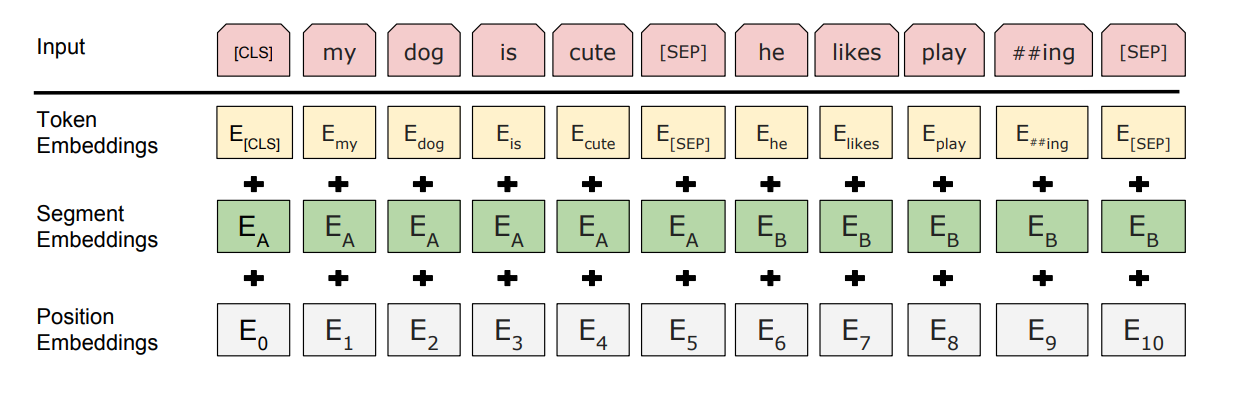
\includegraphics[scale=0.35]{images/bert_embedding_layer.png}
	\caption{BERT Eingabeschicht \cite{BERT:19}}
	\label{embl}
\end{figure}

Aus der Abbildung \ref{embl} kann man nicht nur die Funktion der Schichten lesen, sondern auch ihre Eingaben beobachten. In der Token-Embedding-Schicht werden die Tokens der Wörter gelesen und die Schicht liefert die zugehörige Vektor-Repräsentation. Die Segment-Embedding-Schicht erhält den Segmentenvektor, der bei der Vorverarbeitung der Eingabepaare erstellt wird. Der Positional-Embedding-Layer codiert die Wortindexen in Vektoren. Die Summe der Ergebnisvektoren aus den einzelnen Schichten liefert den eingebetteten Vektor, der die Eingabe im Encoder ist. 

\subsubsection{Optimizer und Loss-Funktion}\label{optimizer_and_loss}
Der nächste Schritt ist die Definition der Optimizer und die Fehlerfunktion. Für den vorliegenden Zweck wird der Adaptive-Movement-Optimizer verwendet. Laut \cite{CO:19} liefern Adam und RMSProp (\textbf{R}oot \textbf{M}ean \textbf{S}quare \textbf{Prop}agation) höhere Richtigkeit und niedrigere Fehlerrate als die anderen Optimizers, wie SGD(\textbf{S}tochastic \textbf{G}radient \textbf{D}escent) und AdaGrad(\textbf{Ada}ptiv \textbf{Gra}dients).  
Bei unserer ersten Task (Masked Language Processing) wird versucht, die maskierten Wörter zu bestimmen. Das impliziert, dass jedes maskierte Wort mehreren Klassen zugehören kann, bzw. aus vielen Wörtern bestehen kann. Aus diesem Grund können nur zwei Fehlerfunktionen verwendet werden, die \textit{CategoricalCrossEntropy} und \textit{SparseCategoricalCrossEntropy} sind.

\textit{CategoricalCrossentropy} ist geeignet, wenn die Ausgabe die partielle Zugehörig-keit zu den Klassen aufweist. Während dessen ist \textit{SparseCategoricalCrossentropy} besser geeignet, wenn die Ausgabe nur einen Integer-Wert beinhaltet bzw. daraus besteht. Dieser Integer stellt die zugehörige Klasse dar. Welche Fehlerfunktion verwendet wird, hängt nur von der Form der Ausgabe ab. Die vorliegende Arbeit beschäftigt sich überwiegend mit \textit{CategoricalCrossEntropy}, da die Ausgaben ein Softmax-Vektor sind. Später wird bei der Anpassung \ref{fine_tuning} wird \textit{SparseCategoricalCrossEntropy} verwendet.

\subsection{Fine-Tuning von einem BERT-Modell}\label{fine_tuning}

Das Modell für das Fine-Tuning wurde dem TensorflowHub \cite{tfhub:21} entnommen. Für diesen Zweck wird ein Modell mit den gleichen Hyperparametern, wie das im Unterkapitel \ref{bert_class} vorgestellte $BERT_{BASE}$ verwendet. Auf TensorflowHub stehen mehrere Modelle zur Wiederverwendung, hier unter anderem BERT-Multilangual-Cased-Modell, BERT-English-uncased, sowohl das Base-BERT-Modell als auch das Large-Modell. Dementsprechend kann das geeignete Modell für die Task ausgewählt werden. Im aktuellen Fall soll ein Translationsmodell aufgebaut werden. Für diesen Zweck wird das Multilingual-BERT-Modell \cite{BERTMM:21} genutzt. 

\subsubsection{BERT-Modell}

Das gelernte BERT-Modell kann wie folgt geladen werden:

\begin{lstlisting}[language=Python, caption={Laden von dem BERT-Modell}]
	# directly from the website
	pre_trained_model = 'https://tfhub.dev/tensorflow/bert_multi_cased_L-12_H-768_A-12/4'
	# or from file system
	pre_train_model_path = 'abs/path/to/Model/dir'
	encoder_input = hub.KerasLayer(pre_trained_model, trainable=True, name="BERT_Encoder")
\end{lstlisting}

Das Modell kann als eine Schicht geladen und somit in dem Modell angefügt werden. Für den Lernprozess braucht das Modell eine weitere Schicht, die die Prognose darstellen soll. Dafür bietet es sich an, eine einfache Dense-Schicht am Modell anzuhängen, die dann die Ausgabe des BERT-Modells mit einem Fully-Connected-Layer verbindet. Die Rolle der Dense-Schicht ist es, die Ausgabe in die richtige Shape zu verwandeln. Die Ausgabe vom BERT-Modell ist ein Vektor mit der Kardinalität \textit{batch\_size} $\times$ \textit{sequence\_length} $\times$ \textit{d\_model}. Die Dense-Schicht transformiert den Ausgabevektor in die Kardinalität \textit{batch\_size} $\times$ \textit{sequence\_length} $\times$ \textit{vocab\_size}. Die $sequence\_length$ entspricht der Länge des Satzes und jeder Index beschreibt ein Wort im Satz. Die Variable \textit{d\_model} repräsentiert die Anzahl der Eigenschaften, nach denen Wörter klassifiziert werden. Die Dense-Schicht verbindet somit die Eingeschaften der einzelnen Wörter zu einem Neuron, wobei die Ausgabe des Neurons ein Wert ist, der für oder gegen ein bestimmtes Wort aus dem Wortschatz spricht. Ein weiterer Schritt ist notwendig, damit diese Werte in Wahrscheinlichkeiten umgewandelt werden können, was nämlich durch die Anwendung der Softmax-Funktion erfolgt. Das heißt, dass das Modell aufgefordert wird, eine Prognose zu erstellen, wie die Übersetzung des Eingabesatzes lauten wird. Hier ist das Modell gegeben:

\begin{lstlisting}[language=Python, label=BERT_Definition, caption={Definition des BERT-Modells zur Anpassung}]
# input Layer with shape=(None, seq_length)
# these are the expected inputs in the BERT model
inputs = dict(
	input_word_ids=tf.keras.layers.Input(shape=(max_sentence_size,), dtype=tf.int32),
	input_mask=tf.keras.layers.Input(shape=(max_sentence_size,), dtype=tf.int32),
	input_type_ids=tf.keras.layers.Input(shape=(max_sentence_size,), dtype=tf.int32)
)
# BERT-Model
encoder_input = hub.KerasLayer(pre_trained_model, trainable=True, name="BERT_Encoder")
outputs = encoder_input(inputs)
net = outputs['sequence_output']
# dropout layer to help prevent overfitting
net = tf.keras.layers.Dropout(0.1)(net)
# dense layer for guessing
output = tf.keras.layers.Dense(vocab_size, activation=None)(net)
# This is our Model
model = tf.keras.Model(inputs, output)
\end{lstlisting}

\subsubsection{Datensatz}
Die Übersetzungstask ähnelt sehr einer Frage-Antwort-Task. Deswegen muss die Datensammlung im Voraus so vorbereitet werden, dass jeder Satz und seine Übersetzung gruppiert werden. Für diese Task wird der Datensatz $\textsc{\textit{/pt\_to\_en}}$ von der Datensatzsammlung $\textit{ted\_hrlr\_translate}$ verwendet. Der Datensatz ist über die Bibliothek $\textit{tensorflow\_datasets}$ zugänglich. Die Datensammlung enthält Sätze auf Englisch und Portugiesisch, also wird das Corpus für die Übersetzung aus dem Englischen ins Portugiesische genutzt. Die Datensammlung besteht jeweils aus 51785 Sätzen in Englisch und Portugiesisch, insgesamt also aus 103570 Sätzen. Die Sätze, die die erlaubte Sequenzlänge überschreiten, werden verworfen. Die ausgewählte Sequenzgröße beträgt 128 Wörter. Da die höhere Satzlänge eine längere Lernzeit bedeutet, wurden in Bezug auf die Hardware, die zur Verfügung steht, eine Sequenzlänge von 128 Wörtern, einschließlich Schlüsselwörter '[CLS]' und '[SEP]', ausgewählt. Das Laden der Datensammlung erfolgt über den folgenden Programmcode:

\begin{lstlisting}[language=Python, caption={Laden der Trainingsdaten}]
	model_name = 'ted_hrlr_translate_pt_en_converter'
	tf.keras.utils.get_file(f"{model_name}.zip", f"https://storage.googleapis.com/download.tensorflow.org/models/{model_name}.zip", cache_dir='.', cache_subdir='', extract=True)
	tokenizer = tf.saved_model.load(model_name)
\end{lstlisting}

Nach der Ausführung des Codes wird die Datensammlung im aktuellen Ordner heruntergeladen und entpackt. Mit Hilfe der dritten Zeile wird der Datensatz zur Nutzung geladen. Der nächste Schritt ist die Vorbereitung der Sätze für den Lernprozess. Hier müssen die Eingaben in einem Dictionary gespeichert werden, da das BERT-Modell so definiert wird. Wie die Eingabe aussieht, ist in der dritten Zeile aus dem Listing \ref{BERT_Definition} zu erkennen.

\subsubsection{Optimizer und Fehlerfunktion}

Als Nächstes werden die Optimizer und die Fehlerfunktion definiert. Für den Optimizer wird Adam verwendet, der über die üblichen Charakteristiken hinaus die Benutzung eines Schedulers für die Lernrate ermöglicht. Das bedeutet, dass die Rate im Laufe des Trainings angepasst werden kann. Die Konfiguration für den Optimizer ist durch den Programmcode gegeben:

\begin{lstlisting}[language=Python, caption={BERT Optimizer}, label=opt_loss]
	from official.nlp import optimization
	# learning rate
	init_lr = 5e-5
	# number steps pro epoch
	steps_per_epoch = len(train_input_array)
	# number of warmup steps
	num_warmup_steps = int(0.1 * steps_per_epoch)
	# the optimizer
	optimizer = optimization.create_optimizer(init_lr=init_lr,
	num_train_steps=steps_per_epoch,
	optimizer_type='adamw')
	# loss function
	tf.keras.losses.SparseCategoricalCrossentropy(from_logits=True)
\end{lstlisting}

Der Optimizer wird durch die Bibliothek \textit{official.nlp.optimization} bereitgestellt. Mit der Einstellung in dem \cref{opt_loss} wird der Optimizer konfiguriert, dass er für \textit{num\_warmup\_steps}-viele Iterationsschritte die Lernrate aufsteigen darf. Nach dem Ablauf der Schritten wird die Lernquote wieder gesunken.

Die genutzte Fehlerfunktion ist SparceCategoricalCrossEntropy. Der Grund dafür ist die Struktur des Labels und die Ausgabe des Modells (siehe Erklärung im Unterkapitel \ref{optimizer_and_loss}). Die Fehlerfunktion hat keine besondere Konfiguration, außer einen Parameter $\textit{from\_logits}$, der auf True gesetzt wird. Dadurch wird für die Fehlerfunktion im Voraus der Befehl vermittelt, dass keine Softmax-Funktion angewendet werden soll. Dementsprechend wird eine Sotfmax-Funktion zuerst ausgeführt, bevor die Fehlerrate errechnet wird.

\chapter{Vektordarstellung}

\section{Einleitung}

Meistens bei der Repräsentation und Analyse einer nummerischen Datensammlung werden die Daten nach bestimmten Kriterien klassifiziert, meistens nach mehr als zwei oder drei, sodass eine Graphische Darstellung relative schwierig zu bilden ist. In der Datenanalyse existieren entsprechende Methoden zur Darstellung von Daten mit mehreren Komponenten. Eins dieser Methode ist Principal Component Analysis (abgekürzt PCA), oder Prizipiele Komponentenanalyse. Diese Methode ist ideal in der NLP zu verwenden, da die Wörter in mehrdimensionalen Vektoren repräsentiert werden, üblicherweise solche mit mehr als drei Komponente. Die Methode verringert die Anzahl der Komponenten auf eine kleinere Zahl, zwei oder drei Dimensionen für eine Darstellung der Wörter im 2D- oder 3D-Raum entsprechend, jedoch so viele Informationen wie möglich über die einzelnen Wörter zu behalten.

\section{Prozess}

Ekläre wie die Berechnung erfolgt und, dass es eine Matrix verändert. Erkläre über DataFrame

\subsubsection{1. Schritt: Standardization}

Im ersten Schritt des PCAs handelt es sich um Standardisierung der Komponenten, sodass jeder gleichmäßig zu der Analyse beibringt. Dieser Schritt ist wichtig, da PCA sehr sinsibel bezüglich Variation der Werte ist. Variablen mit großen Werten dominieren solche mit niedrigen und so ist das Endergebnis beieinflusst/ voreingenommen. Die Standardiesierung erfolgt in Formel:

\begin{equation}
	z_{ij} = \frac{value - mean}{\text{\emph{standard deviation}}},
\end{equation}

Wo \emph{$Z_{ij}$} der normierte Wert mit Zeile \emph{i} und Spalte \emph{j} aus der Matrix ist. Der Meanwert ist der Durchschnitt in einem Vektor und der \" Standard Deviation\" bezieht sich auf dem selben Vektor. Nach der Normierung haben alle Werte der Matrix den selben Maßstab.

\subsubsection{2. Schritt: Berechnung der Kovarianzmatrix}

Nachdem die Normierte Matrix berechnet wurde, wird die Kovarianzmatrix erstellt. Ziel der Kovarainzmatrix ist es die Beziehung zwischen die Variablen zu bestimmen, bzw. wie sie wachsen. Die Abhängigkeit wird von dem Vorzeichen der Covarianzwert bestimmt - bei positivem Wert wachsen die Variablen proporzional und bei negativem - antiproporzional. Die Formel für die Kovarianz ist gegeben:

\begin{equation}
	Cov(X,Y) = \sum \frac{E((X-\mu)(Y - \nu))}{(n - 1)} 
\end{equation}

Die Variable \emph{n} entspricht die Anzahl der Componenten in \emph{X} und in \emph{Y}. Die Zwei konstanten $\mu$ und $\nu$ sind die Durchschnittswerte der beiden Variablen \emph{X} und \emph{Y}. Mit \emph{E} ist der Erwartungswert des Produktes gegeben.

Die Kovarianzmatrix ist eine \emph{p $\times$ p} symmetrische Matrix mit Einträgen als die Corianzwert für alle möglichen Paare, gebildet aus allen Variablen, in diesem Fall normierten Wortvektoren. Zur Darstellung betrachten wir einen Datensatz mit 3 variablen \emph{x}, \emph{y} und \emph{z}. Die Kovarianzmatrix sieht wie folgt aus:

\begin{equation}
\begin{pmatrix}
	Cov(x,x)& & &Cov(x,y)& & &Cov(x,Z)\\
								  \\
	Cov(y,x)& & &Cov(y,y)& & &Cov(y,Z)\\	
                                  \\
	Cov(z,x)& & &Cov(z,y)& & &Cov(z,Z)\\
\end{pmatrix}
\end{equation}

In der Diagonale der Matrix stehen die Werte für Covarianz der Variablen mit sich selbst. Dieser Wert entspricht der Varianz der Variable. Da die Covarianz Kommutative ist, sind die obere und untere Dreiecksmatrix symmetrisch in bezug auf die Diagonale, beziehungsweise gleich.

\subsubsection{3. Berechnung der Eigenvektors und Eigenwerte}

Der nächste Schritt erfordert die Berechnung der Eigenvektors und Eigenwerte der Kovarianzmatrix. Auf diesem Weg bestimmen wir die gesuchten prinzipiellen Komponenten. Diese Komponenten werden als lineare Kombination oder Mischung der Ursprungsvariablen erstellt. Die neuen Variablen sind unabhängig von einander. Der Prozess versucht die meiste Informationen aus allen Variablen in die ersten prinzipiellen Komponenten zu beladen. Das erlaubt es die Dimensionen zu verrigern, ohne große Mengen an Information zu verlieren. Es ist jedoch wichtig zu erwähnen, dass die prinzipiellen Komponenten nicht interpretierbar sind, da sie aus der Linearkombination der alten Variablen berechnet werden.

Geometrisch angesehen die prinzipiellen Komponenten sind Richtungen die einen maximalen Varianzwert darstellen. Das sind Geraden, die die meisten Punkte in einem n-Dimensionalen Raum beschreiben. Die Beziehung zwischen Varianz und Information ist es, dass je größer die Varianz bezüglich einer gegebenen Linie, desto mehr Punkten, bzw. Variable, entlang dieser Linie verteilt sind, umso mehr Information von dieser Linie getragen wird. 

	\begin{figure}
		\centering
		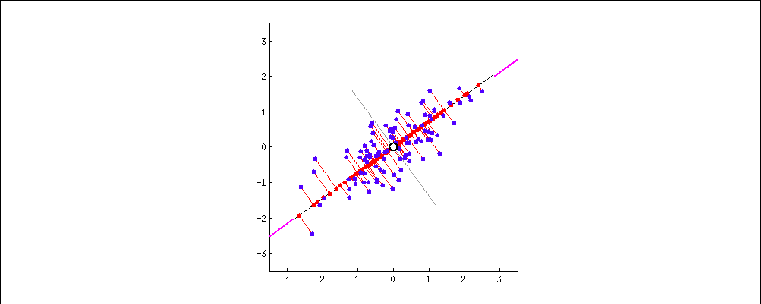
\includegraphics[scale=0.5]{images/PCA_L.png}
		\caption{Prinzipiele Linie}
		\label{PL}
\end{figure}

In der Abbildung \ref{PL} ist die Linie mit der größte Variation und so ist die die erste Prinzipielle Komponente (PK), da sie mit sich die meiste Information trägt. Falls die Variablen dann mit Hilfe dieser PK transformiert werden, wird die meiste Information übertragen. Nachdem die erste Komponente gewählt wird, wird die zweite auf den selben Prinzip gewählt, jedoch wird eine andere Linie gesucht, die dann unabhängig von der erste, meisten eine die Orthogonal zu der Erste liegt. Diese zweite besitzt entsprechend die zweitgrößte Varianz zu den Variablen aus der Datensammlung. Dieser Prozes wiederholt sich bis alle prinzipiellen Komponenten bestimmt sind, oder \emph{p} oft -  genau so oft wie wir Variablen in unsere Kovarianzmatrix haben.

Nun zurück zu den Eigenwerten und -vektoren. Zu Jedem Eigenwert gehört ein Vektor und umgekehrt. Sie Kommen immer in Paare und ihre Anzahl entspricht die dimensionalität der Matrix, wie schon oben erwähnt wurden. Ihre Beziehung in mathematischer Form kann wie folgt dargestellt werden:

\begin{equation}\label{gl1}
	Av = \lambda v,
\end{equation}

wo $\emph{A}$ ist die Matrix, $\emph{v}$ der Eigenvektor und $\lambda$ der zugehörige Eigenwert. Es existiert für eine quadratische Matrix einen Vektor $\emph{v}$ und einen Faktor $\lambda$, sodass bei der Multiplikation der Matrix mit dem Vektor, erhalten wir das gleiche Ergebnis, wie wenn wir den Vektor mit dem Faktor multiplizieren. Es kann die Formel in \ref{gl1} umgeformt werden, um nun die Eigenvektoren und Eigenwerte zu berechnen:

\begin{equation}
	(A - \lambda E).v = 0.
\end{equation}

In der Gleichung enspricht $\emph{E}$ gleich der Einheitsmatrix. Der Eigenvektor ist Lösung der Gleichungssystem. Wir setzte für $\lambda$ den entsprechenden Wert ein und lösen nach v. Jedoch muss der Eigenwert zuerst berechnet werden. Der wird aus der folgenden Formel errechnet:

\begin{equation}
	det(A - \lamda E) = 0
\end{equation}

Wo wir nach den Nullstellen der Determinante suchen. Diese Nullstellen sind die Eingenwerte der Matrix A.

Die Eigenvektoren bestimmen eigentlich die Richtung der Axen mit der meisten Information, oder auch Prinzipielle Komponenten genannt. Die Eingewerte sind die Koeffizienten der Komponente. Je höher der Wert, desto mehr Information wird durch ihre Richtung repräsentiert. Falls die Eigenvektoren nach ihren Eigenwerte absteigend geordnet sind, werden die Ordnung der Prinzipiellen Komponenten bestimmt, sodass die erste Komponente entsprechend diese ist, die den größten Eigenwert besitzt. Als alle Vektoren angeordnet sind, wird einen neuen Vektor aus den zusammengesetzt. Jeder Eigenvektor ist eine Spalte im neuen Vektor. Als nächstes muss die Entscheidung getroffen werden, wie viele prinzipiellen Komponente erhalten werden. Diese Frage hat keine richtige Antwort, in meinem Fall brauche ich nur zwei Komponenten, um die Daten in einem zweidimensionallen Raum darzustellen.


\subsubsection{4. Transformation der Daten}

Im letzten Schritt wird der Prozess abgeschlossen, indem die Ursprungsdaten nach den gefundenen Richtungen ($\emph{Prinzipiellen Komponenten}$), transformiert werden. Die Folgende Formel beschreibt die Operation:

\begin{equation}\label{transPCA}
	T_{L} = V^T_L * Z^T,
\end{equation}  

wo $T_{L}$ die transformierten, $\emph{V}$ enthält die $\emph{L}$ Prinzipiellen Komponenten und $emph{Z}$ beinhaltet den standardisierten Datensatz. Die erhaltene Matrix $\emph{T}$ hat die gewünschte $\emph{L}$ Anzahl an Komponenten. 


QUELLEN:
https://builtin.com/data-science/step-step-explanation-principal-component-analysis

https://royalsocietypublishing.org/doi/10.1098/rsta.2015.0202

https://en.wikipedia.org/wiki/Principal_component_analysis

https://en.wikipedia.org/wiki/Sample_mean_and_covariance

https://www.kaggle.com/jeffd23/visualizing-word-vectors-with-t-sne

https://towardsdatascience.com/visualizing-word-embedding-with-pca-and-t-sne-961a692509f5

https://towardsdatascience.com/visualization-of-word-embedding-vectors-using-gensim-and-pca-8f592a5d3354

https://studyflix.de/mathematik/eigenwert-1635




%\chapter{Weitere Kapitel}

Die Gliederung h�ngt nat�rlich vom Thema und von der L�sungsstrategie ab. Als n�tzliche
Anhaltspunkte k�nnen die Entwicklungsstufen oder - schritte z.B. der Softwareentwicklung betrachtet werden. N�tzliche Gesichtspunkte erh�lt und erkennt man, wenn man sich
\begin{itemize}
  \item in die Rolle des Lesers oder
  \item in die Rolle des Entwicklers, der die Arbeit z.B. fortsetzen, erg�nzen oder pflegen soll,
\end{itemize}
versetzt. In der Regel wird vorausgesetzt, dass die Leser einen fachlichen Hintergrund haben - z.B. Informatik studiert haben. D.h. nur in besonderen, abgesprochenen F�llen schreibt man in popul�rer Sprache, so dass auch Nicht-Fachleute die Ausarbeitung prinzipiell lesen und verstehen k�nnen.

Die �u�ere Gestaltung der Ausarbeitung hinsichtlich Abschnittformate, Abbildungen, mathematische Formeln usw. wird in \hyperref[Stile]{Kapitel~\ref*{Stile}} kurz dargestellt.
%\chapter{LaTeX-Bausteine}\label{Stile}

Der Text wird in bis zu drei Ebenen gegliedert:

\begin{enumerate}
  \item Kapitel ( \verb \chapter{Kapitel} ), \index{Kapitel}
  \item Unterkapitel  ( \verb \section{Abschnitt} ) und
  \item Unterunterkapitel  ( \verb \subsection{Unterabschnitte} ).
\end{enumerate}

\section{Abschnitt}\index{Abschnitt}
Text der Gliederungsebene 2.


\subsection{Unterabschnitt} \index{Unterabschnitt}
Text der Gliederungsebene 3.
Text Text Text Text Text Text Text Text Text Text Text Text Text Text Text
Beispiel f�r Quelltext\index{Quelltext} \\[2 ex]
\noindent
\begin{minipage}{1.0\textwidth} \small
\begin{lstlisting}
	Prozess 1:
	
	Acquire();
		a := 1;
	Release();
	...
	Acquire();
	if(b == 0)
	{					
		c := 3;
		d := a;
	}				
	Release();
\end{lstlisting}
\end{minipage}

\vspace{2cm}
\noindent
\begin{minipage}{1.0\textwidth} \small
\begin{lstlisting}
	Prozess 2:
	
	Acquire();
		b := 1;
	Release();
	...
	Acquire();
	if(a == 0)
	{					
		c := 5;
		d := b;
	}				
	Release();
\end{lstlisting}
\end{minipage}
\vskip 1em

Gr��ere Code-Fragmente sollten im Anhang eingef�gt werden.

\section{Abbildungen und Tabellen}

Abbildung\index{Abbildung} und Tabellen\index{Tabelle} werden zentriert eingef�gt. Grunds�tzlich sollen sie
erst dann erscheinen, nach dem sie im Text angesprochen wurden (siehe Abb. \ref{a1}). Abbildungen und Tabellen (siehe Tabelle \ref{t1}) k�nnen
im (flie�enden) Text (\verb here ), am Seitenanfang (\verb top ), am Seitenende
(\verb bottom ) oder auch gesammelt auf einer nachfolgenden Seite (\verb page )
oder auch ganz am Ende der Ausarbeitung erscheinen. Letzteres sollte man nur
dann w�hlen, wenn die Bilder g�nstig zusammen zu betrachten sind und die
Ausarbeitung nicht zu lang ist ($< 20$ Seiten).

\begin{figure} %[hbtp]
	\centering
		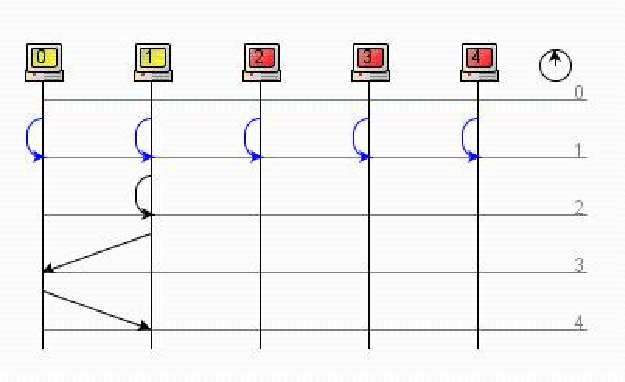
\includegraphics{images/p1ReadSeq.pdf}
	\caption{Bezeichnung der Abbildung}
	\label{a1}
\end{figure}

\begin{table} %[hbtp]
	\centering
		\begin{tabular}{l | l l l l}
		\textbf{Prozesse} & \textbf{Zeit} $\rightarrow$ \\
		\hline
			$P_{1}$ & $W(x)1$ \\
			$P_{2}$ & & $W(x)2$ \\
			$P_{3}$ & & $R(x)2$ & & $R(x)1$\\
			$P_{4}$ & & & $R(x)2$ & $R(x)1$\\
		\end{tabular}
	\caption{Bezeichnung der Tabelle}
	\label{t1}
\end{table}


\section{Mathematische Formel}\index{Formel}
Mathematische Formeln bzw. Formulierungen k�nnen sowohl im
laufenden Text (z.B. $y=x^2$) oder abgesetzt und zentriert im Text
erscheinen. Gleichungen sollten f�r Referenzierungen nummeriert
werden (siehe Formel \ref{gl-1}).
\begin{equation}
\label{gl-1}
e_{i}=\sum _{i=1}^{n}w_{i}x_{i}
\end{equation}

Entscheidungsformel:

\begin{equation}
\psi(t)=\left\{\begin{array}{ccc}
1 &  \qquad 0 <= t < \frac{1}{2} \\
-1 &  \qquad \frac{1}{2} <= t <1 \\
0 & \qquad sonst
\end{array} \right.
\end{equation}


Matrix:\index{Matrix}
\begin{equation}
A = \left(
\begin{array}{llll}
a_{11} & a_{12} & \ldots & a_{1n} \\
a_{21} & a_{22} & \ldots & a_{2n} \\
\vdots & \vdots & \ddots & \vdots \\
a_{n1} & a_{n2} & \ldots & a_{nn} \\
\end{array}
\right)
\end{equation}

Vektor:\index{Vektor} 

\begin{equation}
\overline{a} = \left(
\begin{array}{c}
a_{1}\\
a_{2}\\
\vdots\\
a_{n}\\
\end{array}
\right)
\end{equation}

\section{S�tze, Lemmas und Definitionen}\index{Satz}\index{Lemma}\index{Definition}

S�tze, Lemmas, Definitionen, Beweise,\index{Beweis} Beispiele\index{Beispiel} k�nnen in speziell daf�r vorgesehenen Umgebungen erstellt werden.

\begin{definition}(Optimierungsproblem)

Ein \emph{Optimierungsproblem} $\mathcal{P}$ ist festgelegt durch ein Tupel
$(I_\mathcal{P}, sol_\mathcal{P}, m_\mathcal{P}, goal)$ wobei gilt

\begin{enumerate}
\item $I_\mathcal{P}$ ist die Menge der Instanzen,
\item $sol_\mathcal{P} : I_\mathcal{P} \longmapsto \mathbb{P}(S_\mathcal{P})$ ist eine Funktion, die jeder Instanz $x \in I_\mathcal{P}$ eine Menge zul�ssiger L�sungen zuweist,
\item $m_\mathcal{P} : I_\mathcal{P} \times S_\mathcal{P} \longmapsto \mathbb{N}$ ist eine Funktion, die jedem Paar $(x,y(x))$ mit $x \in I_\mathcal{P}$ und $y(x) \in sol_\mathcal{P}(x)$ eine
Zahl $m_\mathcal{P}(x,y(x)) \in \mathbb{N}$ zuordnet (= Ma� f�r die L�sung $y(x)$ der Instanz $x$), und
\item $goal \in \{min,max\}$.
\end{enumerate}

\end{definition}

\begin{example} MINIMUM TRAVELING SALESMAN (MIN-TSP)
\begin{itemize}
\item $I_{MIN-TSP} =_{def}$ s.o., ebenso $S_{MIN-TSP}$
\item $sol_{MIN-TSP}(m,D) =_{def} S_{MIN-TSP} \cap \mathbb{N}^m$ 
\item $m_{MIN-TSP}((m,D),(c_1, \ldots , c_m)) =_{def} \sum_{i=1}^{m-1} D(c_i, c_{i+1}) + D(c_m,c_1)$ 
\item $goal_{MIN-TSP} =_{def} min$
\end{itemize}
\begin{flushright}
$\qed$
\end{flushright}
\end{example}

\begin{theorem} Sei $\mathcal{P}$ ein \textbf{NP}-hartes Optimierungsproblem.
Wenn $\mathcal{P} \in$ \textbf{PO}, dann ist \textbf{P} = \textbf{NP}.
\end{theorem}

\begin{proof} Um zu zeigen, dass \textbf{P} = \textbf{NP} gilt, gen�gt es
wegen Satz A.30 zu zeigen, dass ein einziges \textbf{NP}-vollst�ndiges
Problem in \textbf{P} liegt. Sei also $\mathcal{P}'$ ein beliebiges \textbf{NP}-vollst�ndiges Problem.

Weil $\mathcal{P}$ nach Voraussetzung \textbf{NP}-hart ist, gilt insbesondere
$\mathcal{P}' \leq_T \mathcal{P}_C$. Sei $R$ der zugeh�rige
Polynomialzeit-Algorithmus dieser Turing-Reduktion.
Weiter ist $\mathcal{P} \in$ \textbf{PO} vorausgesetzt, etwa verm�ge eines
Polynomialzeit-Algorithmus $A$. Aus den beiden
Polynomialzeit-Algorithmen $R$ und $A$ erh�lt man nun
leicht einen effizienten Algorithmus f�r $\mathcal{P}'$: Ersetzt man
in $R$ das Orakel durch $A$, ergibt dies insgesamt eine polynomielle
Laufzeit. 
%\begin{flushright}
$\qed$
% \end{flushright}
\end{proof}

\begin{lemma} Aus \textbf{PO} $=$ \textbf{NPO} folgt \textbf{P} $=$ \textbf{NP}.
\end{lemma}

\begin{proof} Es gen�gt zu zeigen, dass unter der angegeben
Voraussetzung KNAPSACK $\in$ \textbf{P} ist.

Nach Voraussetung ist MAXIMUM KNAPSACK $\in$ \textbf{PO},
d.h. die Berechnung von $m^*(x)$ f�r jede Instanz $x$ ist
in Polynomialzeit m�glich. Um KNAPSACK bei Eingabe
$(x,k)$ zu entscheiden, m�ssen wir nur noch $m^*(x) \geq k$
pr�fen. Ist das der Fall, geben wir $1$, sonst $0$ aus. Dies
bleibt insgesamt ein Polynomialzeit-Algorithmus. 
\begin{flushright}
$\qed$
\end{flushright}
\end{proof}

\section{Fu�noten}

In einer Fu�note k�nnen erg�nzende Informationen\footnote{Informationen die f�r die Arbeit zweitrangig sind, jedoch f�r den Leser interessant sein k�nnten.} angegeben werden. Au�erdem kann eine Fu�note auch Links enthalten. Wird in der Arbeit eine Software (zum Beispiel Java-API\footnote{\url{http://java.sun.com/}}) eingesetzt, so kann die Quelle, die diese Software zur Verf�gung stellt in der Fu�note angegeben werden.

\section{Literaturverweise}\index{Literatur}
Alle benutzte Literatur wird im Literaturverzeichnis angegeben\footnote{Dazu wird ein sogennanter bib-File, literatur.bib verwendet.}. Alle angegebene Literatur sollte mindestens einmal im Text referenziert werden\cite{Coulouris:02}.
%\chapter{Beispiel-Kapitel}

In diesem Kapitel wird beschrieben, warum es unterschiedliche Konsistenzmodelle\index{Konsistenzmodelle} gibt. Au�erdem werden die Unterschiede zwischen strengen Konsistenzmodellen\index{Linearisierbarkeit} (Linearisierbarkeit, sequentielle Konsistenz)\index{sequentiell!Konsistenz} und schwachen Konsistenzmodellen\index{Konsistenz!schwach} (schwache Konsistenz, Freigabekonsistenz)\index{Freigabekonsistenz} erl�utert. Es wird gekl�rt, was Strenge und Kosten (billig, teuer) in Zusammenhang mit Konsistenzmodellen bedeuten.

\section{Warum existieren unterschiedliche Konsistenzmodelle?}

Laut \cite{Malte:97} sind mit der\index{Replikation} Replikation von Daten immer zwei gegens�tzliche Ziele verbunden: die Erh�hung der\index{Verf�gbarkeit} Verf�gbarkeit und die Sicherung der\index{Konsistenz} Konsistenz der Daten. Die Form der Konsistenzsicherung bestimmt dabei, inwiefern das eine Kriterium erf�llt und das andere dementsprechend nicht erf�llt ist (Trade-off zwischen Verf�gbarkeit und der Konsistenz der Daten). Stark konsistente Daten sind stabil, das hei�t, falls mehrere Kopien der Daten existieren, d�rfen keine Abweichungen auftreten. Die Verf�gbarkeit der Daten ist hier jedoch stark eingeschr�nkt. Je schw�cher die Konsistenz wird, desto mehr Abweichungen k�nnen zwischen verschiedenen Kopien einer Datei auftreten, wobei die Konsistenz nur an bestimmten Synchronisationspunkten gew�hrleistet wird. Daf�r steigt aber die Verf�gbarkeit der Daten, weil sie sich leichter replizieren lassen.

Nach \cite{Mosberger:93} kann die Performanzsteigerung der schw�cheren Konsistenzmodelle wegen der Optimierung\index{Optimierung} (Pufferung, Code-Scheduling, Pipelines) 10-40 Prozent betragen. Wenn man bedenkt, dass mit der Nutzung der vorhandenen Synchronisierungsmechanismen schw�chere Konsistenzmodelle den Anforderungen der strengen Konsistenz gen�gen, stellt sich der h�here programmiertechnischer Aufwand bei der Implementierung der schw�cheren Konsistenzmodelle als ihr einziges Manko dar.

In \cite{Cheriton:85} ist beschrieben, wie man sich Formen von DSM vorstellen k�nnte, f�r die ein beachtliches Ma� an\index{Inkonsistenz} Inkonsistenz akzeptabel w�re. Beispielsweise k�nnte DSM verwendet werden, um die Auslastung von Computern in einem Netzwerk zu speichern, so dass Clients f�r die Ausf�hrung ihrer Applikationen die am wenigsten ausgelasteten Computer ausw�hlen k�nnen. Weil die Informationen dieser Art innerhalb k�rzester Zeit ungenau werden k�nnen (und durch die Verwendung der veralteten Daten keine gro�en Nachteile entstehen k�nnen), w�re es vergebliche M�he, sie st�ndig f�r alle Computer im System konsistent zu halten \cite{Coulouris:02}. Die meisten Applikationen stellen jedoch strengere Konsistenzanforderungen.

\section{Klassifizierung eines Konsistenzmodells}

Die zentrale Frage, die f�r die Klassifizierung\index{streng}\index{schwach} (streng oder schwach) eines Konsistenzmodells von Bedeutung ist \cite{Coulouris:02}: wenn ein Lesezugriff auf eine Speicherposition erfolgt, welche Werte von Schreibzugriffen auf diese Position sollen dann dem Lesevorgang bereitgestellt werden? Die Antwort f�r das schw�chste Konsistenzmodell lautet: von jedem Schreibvorgang, der vor dem Lesen erfolgt ist, oder in der "`nahen"' Zukunft, innerhalb des definierten Betrachtungsraums, erfolgten wird. Also irgendein Wert, der vor oder nach dem Lesen geschrieben wurde.

F�r das strengste Konsistenzmodell, Linearisierbarkeit (atomic consistency), stehen alle geschriebenen Werte allen Prozessoren sofort zur Verf�gung: eine Lese-Operation gibt den aktuellsten Wert zur�ck, der geschrieben wurde, bevor das Lesen stattfand. Diese Definition ist aber in zweierlei Hinsicht problematisch. Erstens treten weder Schreib- noch Lese-Operationen zu genau einem Zeitpunkt auf, deshalb ist die Bedeutung von "`aktuellsten"' nicht immer klar. Zweitens ist es nicht immer m�glich, genau festzustellen, ob ein Ereignis vor einem anderen stattgefunden hat, da es Begrenzungen daf�r gibt, wie genau Uhren in einem verteilten System synchronisiert werden k�nnen.

Nachfolgend werden einige Konsistenzmodelle absteigend nach ihrer Strenge vorgestellt. Zuvor m�ssen wir allerdings kl�ren, wie die Lese- und Schreibe-Operationen in dieser Ausarbeitung dargestellt werden.

Sei $x$ eine Speicherposition, dann k�nnen Instanzen dieser Operationen wie folgt ausgedr�ckt werden:
\begin{itemize}
	\item $R(x)a$ - eine Lese-Operation\index{Operation!Lese}, die den Wert $a$ von der Position $x$ liest.
	\item $W(x)b$ - eine Schreib-Operation\index{Operation!Schreib}, die den Wert $b$ an der Position $x$ speichert.
\end{itemize}

\section{Linearisierbarkeit\index{Linearisierbarkeit} (atomic consistency)}

Die Linearisierbarkeit im Zusammenhang mit DSM kann wie folgt definiert werden:
\begin{itemize}
	\item Die verzahnte Operationsabfolge findet so statt: wenn $R(x)a$ in der Folge vorkommt, dann ist die letzte Schreib-Operation, die vor ihr in der verzahnten Abfolge auftritt, $W(x)a$, oder es tritt keine Schreib-Operation vor ihr auf und $a$ ist der Anfangswert von $x$. Das bedeutet, dass eine Variable nur durch eine Schreib-Operation ge�ndert werden kann.
	\item Die Reihenfolge der Operationen in der Verzahnung ist konsistent zu den \underline{Echtzeiten}\index{Echtzeiten}, zu denen die Operationen bei der tats�chlichen Ausf�hrung aufgetreten sind.
\end{itemize}

Die Bedeutung dieser Definition kann an folgendem Beispiel (Tabelle \ref{tab:1}) nachvollzogen werden. Es sei angenommen, dass alle Werte mit $0$ vorinitialisiert sind.

\begin{table}
	\centering
		\begin{tabular}{l | l l l l}
			\textbf{Prozesse} & \textbf{Zeit} $\rightarrow$ & \\
			\hline
			$P_{1}$ & $W(x)1$ & & $W(y)2$ \\
			$P_{2}$ & & $R(x)1$ & & $R(y)2$ \\
		\end{tabular}
	\caption{Linearisierbarkeit ist erf�llt}
	\label{tab:1}
\end{table}

Hier sind beide Bedingungen erf�llt, da die Lese-Operationen den zuletzt geschriebenen Wert zur�ckliefern. Interessanter ist es, zu sehen, wann die Linearisierbarkeit verletzt ist.

\begin{table}
	\centering
		\begin{tabular}{l | l l l l}
		\textbf{Prozesse} & \textbf{Zeit} $\rightarrow$ \\
		\hline
		$P_{1}$ & $W(x)1$ & $W(x)2$ \\
		$P_{2}$ & & & \color{red} $R(x)0$ & \color{black} $R(x)2$ \\
		\end{tabular}
	\caption{Linearisierbarkeit ist verletzt, sequentielle Konsistenz ist erf�llt.}
	\label{tab:2}
\end{table}

In diesem Beispiel (Tabelle \ref{tab:2}) ist die Echtzeit-Anforderung verletzt, da der Prozess $P_{2}$ immer noch den alten Wert liest, obwohl er von Prozess $P_{1}$ bereits ge�ndert wurde. Diese Ausf�hrung w�re aber sequentiell konsistent (siehe kommender Abschnitt), da es eine Verzahnung der Operationen gibt, die diese Werte liefern k�nnte ($R(x)0$, $W(x)1$, $W(x)2$, $R(y)2$). W�rde man beide Lese-Operationen des 2. Prozesses vertauschen, wie in der Tabelle \ref{tab:3} dargestellt, so w�re keine sinnvolle Verzahnung mehr m�glich.

\begin{table}
	\centering
		\begin{tabular}{l | l l l l}
		\textbf{Prozesse} & \textbf{Zeit} $\rightarrow$ \\
		\hline
		$P_{1}$ & $W(x)1$ & $W(x)2$ \\
		$P_{2}$ & & & \color{red} $R(x)2$ &  \color{red} $R(x)0$ \\
			
		\end{tabular}
	\caption{Linearisierbarkeit und sequentielle Konsistenz sind verletzt.}
	\label{tab:3}
\end{table}

In diesem Beispiel sind beide Bedingungen verletzt. Selbst wenn die Echtzeit, zu der die Operationen stattgefunden haben, ignoriert wird, gibt es keine Verzahnung einzelner Operationen, die der Definition entsprechen w�rde.
\chapter{Zusammenfassung und Ausblick}

In diesem Kapitel soll die Arbeit noch einmal kurz zusammengefasst werden. Insbesondere sollen die wesentlichen Ergebnisse Ihrer Arbeit herausgehoben werden. Erfahrungen, die z.B. Benutzer mit der Mensch-Maschine-Schnittstelle gemacht haben oder Ergebnisse von Leistungsmessungen sollen an dieser Stelle pr�sentiert werden. Sie k�nnen in diesem Kapitel auch die Ergebnisse oder das Arbeitsumfeld Ihrer Arbeit kritisch bewerten. W�nschenswerte Erweiterungen sollen als Hinweise auf weiterf�hrende Arbeiten erw�hnt werden.
% ...
%--------------------------------------------------------------------------
\backmatter                        		% Anhang
%-------------------------------------------------------------------------
\bibliographystyle{geralpha}			% Literaturverzeichnis
\bibliography{literatur}     			% BibTeX-File literatur.bib
%--------------------------------------------------------------------------
\printindex 							% Index (optional)
%--------------------------------------------------------------------------
\begin{appendix}						% Anh�nge sind i.d.R. optional
   \chapter{Glossar}

\abbreviation{DisASTer}		{DisASTer (Distributed Algorithms Simulation Terrain), A platform for the Implementation of Distributed Algorithms}
\abbreviation{DSM}			{Distributed Shared Memory}
\abbreviation{AC}			{Linearisierbarkeit (atomic consistency)}
\abbreviation{SC}			{Sequentielle Konsistenz (sequential consistency)}
\abbreviation{WC}			{Schwache Konsistenz (weak consistency)}
\abbreviation{RC}			{Freigabekonsistenz (release consistency)}
			% Glossar   
   \inputencoding{latin1}
\chapter{Erkl�rung der Kandidatin / des Kandidaten}

\begin{description}[$\Box$~]
\item[$\Box$] Die Arbeit habe ich selbstst�ndig verfasst und keine anderen als die angegebenen Quellen- und Hilfsmittel verwendet.\\

\item[$\Box$] Die Arbeit wurde als Gruppenarbeit angefertigt. Meine eigene Leistung ist\\
...\\

Diesen Teil habe ich selbstst�ndig verfasst und keine anderen als die angegebenen Quellen und Hilfsmittel verwendet. \\

\end{description}

\vspace{2cm}

\begin{minipage}[t]{3cm}
\rule{3cm}{0.5pt}
Datum
\end{minipage}
\hfill
\begin{minipage}[t]{9cm}
\rule{9cm}{0.5pt}
Unterschrift der Kandidatin / des Kandidaten
\end{minipage}
   	% Selbstst�ndigkeitserkl�rung
\end{appendix}

\end{document}
